\setcounter{dang}{0}
\setcounter{section}{2}
\section{Dấu của tam thức bậc hai}
\subsection{Tóm tắt lý thuyết}
	\subsubsection{Dấu của tam thức bậc hai}
	\begin{dn}{}
	Tam thức bậc hai là biểu thức có dạng $f(x) = ax^2 + bx + c,$ trong đó $a,b,c$ là những hệ số, $a\ne 0$. Nghiệm của tam thức bậc hai là giá trị của $x$ làm cho tam thức có giá trị bằng $0$.
	\end{dn}
	%	\subsubsection{Định lí về dấu của tam thức bậc hai}
	\begin{dl}{[Định lí về dấu của tam thức bậc hai]}
	Cho tam thức bậc hai $f(x) = ax^2 + bx + c,a\ne 0,\Delta = b^2 - 4ac$.
	Khi đó:
	\begin{itemize}
	\item $\Delta < 0\Rightarrow af(x) > 0,\forall x\in \mathbb{R}$.
	\item $ \Delta = 0\Rightarrow af(x) > 0,\forall x\in \mathbb{R}\backslash \left\{ - \dfrac{b}{2a}\right\} $ và $f\left(-\dfrac{b}{2a}\right)=0$.
	\item $ \Delta > 0\Rightarrow \hoac{
	& af(x) > 0,\forall x\in (-\infty; x_1)\cup (x_2; +\infty) \\ 
	& af(x) < 0,\forall x\in (x_1; x_2).}$
	\end{itemize}
	Với $x_1;x_2$ là nghiệm của phương trình $f(x) = 0$, $x_1 < x_2$.
	\end{dl}
	\subsubsection{Bất phương trình bậc hai}
	\begin{dn}{}
	Bất phương trình bậc hai một ẩn số là bất phương trình có dạng $ax^2 + bx + c > 0$ (hoặc $ax^2 + bx + c > 0; ax^2 + bx + c\ge 0; ax^2 + bx + c\le 0)$ với $a,b,c$ là những số thực đã cho, $a\ne 0$, $x$ là ẩn số.
	\end{dn}
\subsection{Các dạng toán}
%Dạng 1
\begin{dang}{Nhận dạng và xét dấu của tam thức bậc hai}
	Đa thức bậc hai $f(x)=ax^2+bx+c$ với $a$, $b$, $c$ là các hệ số, $a\ne 0$ và $x$ là biến số thực gọi là tam thức bậc hai.\\
	Phương pháp xét dấu của tam thức bậc hai $f(x)=ax^2+bx+c$\\
	Bước 1: Tính và xác định dấu của biệt thức $\Delta=b^2-4ac$.\\
	Bước 2: Xác định nghiệm của $f(x)$ (nếu có).\\
	Bước 3: Xác định dấu của hệ số $a$.\\
	Bước 4: Xác định dấu của $f(x)$.\\
	Nếu $\Delta <0$ thì $f(x)$ cùng dấu với $a$ với mọi giá trị $x$.\\
	Nếu $\Delta =0$ và $x=-\dfrac{b}{2a}$ là nghiệm kép của $f(x)$ thì $f(x)$ cùng dấu với $a$ với mọi $x$ khác $x_0$.\\
	Nếu $\Delta>0$ và $x_1$, $x_2$ là hai nghiệm của $f(x)$ $(x_1<x_2)$ thì $f(x)$ trái dấu với $a$ với mọi $x$ thuộc khoảng $(x_1;x_2)$ và $f(x)$ cùng dấu với $a$ với mọi $x$ thuộc hai khoảng $(-\infty;+\infty)$.
\end{dang}
\viduminhhoa
\begin{vd}%[Đoàn Minh Tân]%[0D4Y5-1]
	Đa thức nào sau đây là tam thức bậc hai?
	\begin{listEX}[3]
	\item $4x^2+3x+1$.
	\item $x^3+3x^2-1$.
	\item $2x^2+4x-1$.
	\end{listEX}
\loigiai{
	Tam thức bậc hai là đa thức có dạng $f(x)=ax^2+bx+c$ với $a\ne 0$.\\
	Do đó các đa thức $4x^2+3x+1$ và $2x^2+4x-1$ là các tam thức bậc hai.\\
	Đa thức $x^3+3x^2-1$ có một hạng tử là $x^3$ nên không là tam thức bậc hai.
	}
\end{vd}
\newpage
\begin{vd}%[Đoàn Minh Tân]%[0D4B5-1]
	Xác định giá trị của tham số $m$ để các đa thức sau là tam thức bậc hai.
	\begin{listEX}[3]
	\item $(m+1)x^2+2x+m$.
	\item $mx^3+2x^2-x+m$.
	\item $-5x^2+2x-m+1$.
	\end{listEX}
	\loigiai{
	\begin{enumerate}
	\item Đa thức $(m+1)x^2+2x+m$ là tam thức bậc hai khi và chỉ khi $m+1\ne 0\Leftrightarrow m\ne -1$.
	\item Đa thức $mx^3+2x^2-x+m$ là tam thức bậc hai khi và chỉ khi $m=0$.
	\item Đa thức $-5x^2+2x-m+1$ luôn là tam thức bậc hai với mọi $m\in \mathbb{R}$.
	\end{enumerate}
	}
\end{vd}
% \begin{vd}%[Đoàn Minh Tân]%[0D4Y5-1]
% 	Cho tam thức bậc hai $f(x)=3x^2+4x-7$.
% 	\begin{enumerate}
% 	\item Tính biệt thức và nghiệm (nếu có) của $f(x)$.
% 	\item Xác định dấu của $f(x)$ tại $x=0$ và $x=3$.
% 	\end{enumerate}
% 	\loigiai{
% 	\begin{enumerate}
% 	\item Ta có $\Delta =4^2-4\cdot 3\cdot (-7)=100>0$.\\
% 	Do đó $f(x)$ có hai nghiệm $x_1=-\dfrac{7}{3}$ và $x_2=1$.
% 	\item $f(0)=-7<0$, $f(3)=32>0$.
% 	\end{enumerate}
% 	}
% \end{vd}
\begin{vd}%[Đoàn Minh Tân]%[0D4B5-1]
	Tìm các giá trị của tham số $m$ để biểu thức $f(x)=\left(m^2-1\right)x^2+3mx-6$ là một tam thức bậc hai có $x=2$ là một nghiệm.
	\loigiai{
	Ta có $f(x)$ là một tam thức bậc hai khi và chỉ khi $m^2-1\ne 0\Leftrightarrow m\ne 1$ và $m\ne -1$.\\
	Do $x=2$ là một nghiệm của $f(x)$ nên $f(2)=0$
	$$\Leftrightarrow 4\left(m^2-1\right)+6m-6=0\Leftrightarrow 4m^2+6m-10=0\Leftrightarrow \hoac{& m=1&\text{(loại)}\\ & m=-\dfrac{5}{2} & \text{(nhận)}.}$$
	Vậy $m=-\dfrac{5}{2}$.
	}
\end{vd}
\begin{vd}%[Đoàn Minh Tân]%[0D4Y5-1]
	Xét dấu của các tam thức bậc hai sau
	\begin{listEX}[3]
	\item $f(x)=2x^2+4x+2$.
	\item $f(x)=-3x^2+2x+21$.
	\item $f(x)=-2x^2-x-2$.
	\item $f(x)=-4x(x+3)-9$.
	\item $f(x)=(2x+5)(x-3)$.
	\end{listEX}
	\loigiai{
	\begin{enumerate}
	\item $f(x)=2x^2+4x+2$ có $\Delta =0$, nghiệm kép là $x_0=-1$ và $a=2>0$.\\
	Vậy $f(x)>0$ với mọi $x\ne -1$.
	\item $f(x)=-3x^2+2x+21$ có $\Delta=256$, hai nghiệm phân biệt là $x_1=-\dfrac{7}{3}$ và $x_2=3$, hệ số $a=-3<0$.\\
	Ta có bảng xét dấu của $f(x)$ như sau
	\begin{center}
	
\begin{tikzpicture}
	\tkzTabInit[nocadre=false, lgt=1.5, espcl=3]
	{$x$ /1,$f(x)$ /0.6}
	{$-\infty$, $-\dfrac{7}{3}$,$3$, $+\infty$}
	\tkzTabLine{,-,0,+,0,-}
	\end{tikzpicture}
	\end{center}
	Từ bảng xét dấu, suy ra $f(x)<0\Leftrightarrow x\in \left(-\infty;-\dfrac{7}{3}\right)\cup (3;+\infty)$;\\
	$f(x)>0\Leftrightarrow x\in \left(-\dfrac{7}{3};3\right)$.
	\item $f(x)=-2x^2-x-2$ có $\Delta =-15<0$ và $a=-2<0$ nên $f(x)$ luôn âm với mọi $x\in \mathbb{R}$.
	\item $f(x)=-4x(x+3)-9=-4x^2-12x-9$ có $\Delta=0$, nghiệm kép $x_0=-\dfrac{3}{2}$ và hệ số $a=-4<0$.\\
	Do đó $f(x)<0$ với mọi $x\ne -\dfrac{3}{2}$.
	\item $f(x)=(2x+5)(x-3)=2x^2-x-15$ có $\Delta=121>0$, hai nghiệm $x_1=-\dfrac{5}{2}$, $x_2=3$ và hệ số $a=2>0$\\
	Ta có bảng xét dấu của $f(x)$ như sau
	\begin{center}
	
\begin{tikzpicture}
	\tkzTabInit[nocadre=false, lgt=1.5, espcl=3]
	{$x$ /1,$f(x)$ /0.6}
	{$-\infty$, $-\dfrac{5}{2}$,$3$, $+\infty$}
	\tkzTabLine{,+,0,-,0,+}
	\end{tikzpicture}
	\end{center}
	Từ bảng xét dấu, suy ra $f(x)>0\Leftrightarrow x\in \left(-\dfrac{5}{2};3\right)$;\\
	$f(x)>0\Leftrightarrow x\in \left(-\infty;-\dfrac{5}{2}\right)\cup (3;+\infty)$.
	\end{enumerate}	
	}
\end{vd}
\begin{vd}%[Đoàn Minh Tân]%[0D4B5-1]
	Dựa vào đồ thị của các hàm số bậc hai sau, hãy lập bảng xét dấu của tam thức bậc hai tương ứng.
	\begin{enumerate}
	\item \immini
	{
	$f(x)=x^2+1{,}5x-1$.
	}
	{
	\begin{tikzpicture}[scale=.6, font=\footnotesize, line join=round, line cap=round,>=stealth]
	\def \xmin{-3};
	\def \xmax{2};
	\def \ymin{-2};
	\def \ymax{3};
	\draw[->] (\xmin, 0.) -- (\xmax,0.) node[anchor=north] {$x$};
	\draw[->] (0.,\ymin) -- (0.,\ymax) node[anchor=west] {$y$};
	\clip(\xmin-0.1,\ymin-0.1) rectangle (\xmax+0.1,\ymax+0.1);
	\draw[smooth] plot[domain=\xmin:\xmax] (\x,{(\x)^2+1.5*(\x)-1});
	\draw[fill=black] (-2,0) circle(1pt) node[below left]{$-2$} (0,0) circle(1pt) node[below left]{$O$} (0.5,0) circle(1pt) node[below]{$\tfrac{1}{2}$};
	\end{tikzpicture}
	}
	\item \immini
	{
	$f(x)=-0{,}5x^2+3x-6$.
	}
	{
	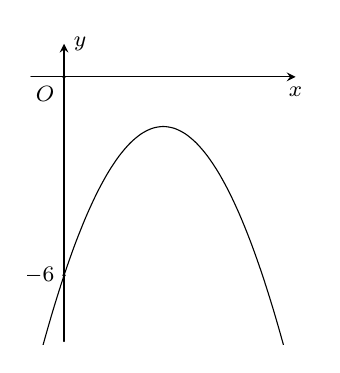
\begin{tikzpicture}[scale=0.6, font=\footnotesize, xscale=0.7, yscale=0.7,line join=round, line cap=round,>=stealth]
	\def \xmin{-1};
	\def \xmax{7};
	\def \ymin{-8};
	\def \ymax{1};
	\draw[->] (\xmin, 0.) -- (\xmax,0.) node[anchor=north] {$x$};
	\draw[->] (0.,\ymin) -- (0.,\ymax) node[anchor=west] {$y$};
	\clip(\xmin-0.1,\ymin-0.1) rectangle (\xmax+0.1,\ymax+0.1);
	\draw[smooth] plot[domain=\xmin:\xmax] (\x,{-0.5*(\x)^2+3*(\x)-6});
	\draw[fill=black] (0,0) circle(1pt) node[below left]{$O$} (0,-6) circle(1pt) node[left]{$-6$};
	\end{tikzpicture}
	}
	\item \immini
	{
	$f(x)=x^2+2x+1$.
	}
	{
	\begin{tikzpicture}[scale=0.6, font=\footnotesize,line join=round, line cap=round,>=stealth]
	\def \xmin{-4};
	\def \xmax{2};
	\def \ymin{-1};
	\def \ymax{5};
	\draw[->] (\xmin, 0.) -- (\xmax,0.) node[anchor=north] {$x$};
	\draw[->] (0.,\ymin) -- (0.,\ymax) node[anchor=west] {$y$};
	\clip(\xmin-0.1,\ymin-0.1) rectangle (\xmax+0.1,\ymax+0.1);
	\draw[smooth] plot[domain=\xmin:\xmax] (\x,{(\x)^2+2*(\x)+1});
	\draw[fill=black] (0,0) circle(1pt) node[below right]{$O$} (-1,0) circle(1pt) node[below]{$-1$};
	\end{tikzpicture}
	}
	\end{enumerate}
	\loigiai{
	Từ các đồ thị, ta có bảng xét dấu của các tam thức bậc hai như sau
	\begin{enumerate}
	\item \hfill
	\begin{center}
	
\begin{tikzpicture}
	\tkzTabInit[nocadre=false, lgt=1.5, espcl=3]
	{$x$ /1,$f(x)$ /0.6}
	{$-\infty$, $-2$,$\dfrac{1}{2}$, $+\infty$}
	\tkzTabLine{,+,0,-,0,+}
	\end{tikzpicture}
	\end{center}
	\item \hfill
	\begin{center}
	
\begin{tikzpicture}
	\tkzTabInit[nocadre=false, lgt=1.5, espcl=3]
	{$x$ /0.6,$f(x)$ /0.6}
	{$-\infty$, $+\infty$}
	\tkzTabLine{,-}
	\end{tikzpicture}
	\end{center}
	\item \hfill
	\begin{center}
	
\begin{tikzpicture}
	\tkzTabInit[nocadre=false, lgt=1.5, espcl=3]
	{$x$ /1,$f(x)$ /0.6}
	{$-\infty$, $-1$, $+\infty$}
	\tkzTabLine{,+,0,+}
	\end{tikzpicture}
	\end{center}
	\end{enumerate}
	}
\end{vd}
\baitaptl
\begin{bt}%[Đoàn Minh Tân]%[0D4Y5-1]
	Xét dấu của mỗi tam thức bậc hai sau
	\begin{enumerate}
	\item $f(x)=3x^2-4x+1$.
	\item $f(x)=9x^2+6x+1$.
	\item $f(x)=2x^2-3x+10$.
	\item $f(x)=-5x^2+2x+3$.
	\item $f(x)=-4x^2+8x-4$.
	\item $f(x)=-3x^2+3x-1$.
	\end{enumerate}
	\loigiai{
	\begin{enumerate}
	\item $f(x)=3x^2-4x+1$ có $\Delta=4>0$, hai nghiệm $x_1=\dfrac{1}{3}$, $x_2=1$ và hệ số $a>3>0$.\\
	Bảng xét dấu của $f(x)$
	\begin{center}
	
\begin{tikzpicture}
	\tkzTabInit[nocadre=false, lgt=1.5, espcl=3]
	{$x$ /1,$f(x)$ /0.6}
	{$-\infty$, $\dfrac{1}{3}$,$1$, $+\infty$}
	\tkzTabLine{,+,0,-,0,+}
	\end{tikzpicture}
	\end{center}
	Dựa vào bảng xét dấu, suy ra
	$f(x)>0\Leftrightarrow x\in \left(-\infty;\dfrac{1}{3}\right)\cup (1;+\infty)$.\\
	$f(x)<0\Leftrightarrow x\in \left(\dfrac{1}{3};1\right)$.
	\item $f(x)=9x^2+6x+1$ có $\Delta=0$, nghiệm kép $x=-\dfrac{1}{3}$ và hệ số $a=9>0$.\\
	Do đó $f(x)>0$ với mọi $x\ne -\dfrac{1}{3}$.
	\item $f(x)=2x^2-3x+10$ có $\Delta =-71<0$ và hệ số $a=2>0$ nên $f(x)>0$ với mọi $x\in \mathbb{R}$.
	\item $f(x)=-5x^2+2x+3$ có $\Delta=64>0$, hai nghiệm $x_1=-\dfrac{3}{5}$, $x_2=1$ và hệ số $a=-5<0$.\\
	Bảng xét dấu của $f(x)$
	\begin{center}
	
\begin{tikzpicture}
	\tkzTabInit[nocadre=false, lgt=1.5, espcl=3]
	{$x$ /1,$f(x)$ /0.6}
	{$-\infty$, $-\dfrac{3}{5}$,$1$, $+\infty$}
	\tkzTabLine{,-,0,+,0,-}
	\end{tikzpicture}
	\end{center}
	Dựa vào bảng xét dấu, suy ra\\
	$f(x)<0\Leftrightarrow x\in \left(-\infty;-\dfrac{3}{5}\right)\cup (1;+\infty)$.\\
	$f(x)>0\Leftrightarrow x\in \left(-\dfrac{3}{5};1\right)$.
	\item $f(x)=-4x^2+8x-4$ có $\Delta=0$, nghiệm kép $x=1$ và hệ số $a=-4<0$.\\
	Do đó $f(x)<0$ với mọi $x\ne 1$.
	\item $f(x)=-3x^2+3x-1$ có $\Delta=-3<0$ và hệ số $a=-3<0$ nên $f(x)<0$ với mọi $x\in \mathbb{R}$.
	\end{enumerate}
	}
\end{bt}
\begin{bt}%[Đoàn Minh Tân]%[0D4Y5-1]
	Tính biệt thức và nghiệm (nếu có) của các tam thức bậc hai. Xác định dấu của chúng tại $x=-2$.
	\begin{enumerate}
	\item $f(x)=-2x^2+3x-4$.
	\item $g(x)=2x^2+8x+8$.
	\item $h(x)=3x^2+7x-10$.
	\end{enumerate}
	\loigiai{
	\begin{enumerate}
	\item $f(x)=-2x^2+3x-4$ có $\Delta=-23<0$ nên $f(x)$ vô nghiệm.\\
	Lại có $f(-2)=-18<0$.
	\item $g(x)=2x^2+8x+8$ có $\Delta =0$ nên $g(x)$ có nghiệm kép $x=-2$.\\
	Do đó $g(-2)=0$.
	\item $h(x)=3x^2+7x-10$ có $\Delta=169>0$ nên $g(x)$ có hai nghiệm $x_1=-\dfrac{10}{3}$ và $x_2=1$.\\
	Lại có $h(-2)=-12<0$.
	\end{enumerate}	
	}
\end{bt}
\begin{bt}%[Đoàn Minh Tân]%[0D4B5-1]
	Tìm tham số $m$ để
	\begin{enumerate}
	\item $f(x)=(2m-8)x^2+2mx+1$ là một tam thức bậc hai.
	\item $f(x)=(2m+3)x^2+3x-4m^2$ là một tam thức bậc hai có $x=3$ là một nghiệm.
	\item $f(x)=2x^2+mx-3$ dương tại $x=2$.
	\end{enumerate}
	\loigiai{
	\begin{enumerate}
	\item $f(x)=(2m-8)x^2+2mx+1$ là một tam thức bậc hai khi và chỉ khi
	$$2m-8\ne 0\Leftrightarrow m\ne 4.$$
	\item $f(x)=(2m+3)x^2+3x-4m^2$ là một tam thức bậc hai khi và chỉ khi
	$$2m+3\ne 0\Leftrightarrow m\ne -\dfrac{3}{2}.$$
	Do $x=3$ là một nghiệm của $f(x)$ nên $f(3)=0$
	$$\Leftrightarrow 9(2m+3)+9-4m^2=0\Leftrightarrow -4m^2+18m+36=0\Leftrightarrow \hoac{& m=6 & \text{(nhận)}\\ & m=-\dfrac{3}{2} & \text{(loại)}.}$$
	Vậy $m=6$.
	\item $f(x)=2x^2+mx-3$ dương tại $x=2$
	$$\Leftrightarrow f(2)>0\Leftrightarrow 8+2m-3>0\Leftrightarrow m>-\dfrac{5}{2}.$$
	\end{enumerate}
	}
\end{bt}
\begin{bt}%[Đoàn Minh Tân]%[0D4B5-1]
	Tìm các giá trị của tham số $m$ để 
	\begin{enumerate}
	\item $f(x)=\left(m^2+9\right)x^2+(m+6)x+1$ là một tam thức bậc hai có một nghiệm duy nhất.
	\item $f(x)=(m-1)x^2+3x+1$ là một tam thức bậc hai có hai nghiệm phân biệt.
	\item $f(x)=mx^2+(m+2)x+1$ là một tam thức bậc hai vô nghiệm.
	\end{enumerate}
	\loigiai{
	\begin{enumerate}
	\item $f(x)=\left(m^2+9\right)x^2+(m+6)x+1$ luôn một tam thức bậc hai do $m^2+9\ne 0,\, \forall x\in \mathbb{R}$.\\
	$f(x)$ có nghiệm duy nhất $\Leftrightarrow \Delta =0 \Leftrightarrow (m+6)^2-4\left(m^2+9\right)=0\Leftrightarrow -3m^2+12m=0\Leftrightarrow \hoac{& m=0\\ & m=4.}$\\
	Vậy $m=0$ và $m=4$ thì $f(x)$ là tam thức bậc hai có nghiệm duy nhất.
	\item $f(x)=(m-1)x^2+3x+1$ là một tam thức bậc hai khi và chỉ khi $m-1\ne 0\Leftrightarrow m\ne 1$.\\
	$f(x)$ có hai nghiệm phân biệt $\Leftrightarrow \Delta>0\Leftrightarrow 9-4(m-1)>0\Leftrightarrow m<\dfrac{13}{4}.$\\
	Vậy $m\in \left(-\infty;\dfrac{13}{4}\right)\setminus \{1\}$.
	\item $f(x)=mx^2+(m+2)x+1$ là một tam thức bậc hai khi và chỉ khi $m\ne 0$.\\
	$f(x)$ vô nghiệm $\Leftrightarrow \Delta <0\Leftrightarrow (m+2)^2-4m<0\Leftrightarrow m^2+4<0$ (vô lí).\\
	Do đó không tìm được $m$.
	\end{enumerate}	
	}
\end{bt}
%\begin{bt}%[Đoàn Minh Tân]%[0D4B5-1]
%	Tìm nghiệm và lập bảng xét dấu của tam thức bậc hai $f(x)$ với đồ thị được cho ở mỗi hình sau
%	\begin{enumerate}
%	\item 
%	\begin{tikzpicture}[scale=1, xscale=0.5, yscale=0.3,font=\footnotesize,line join=round, line cap=round,>=stealth]
%	\def \xmin{-4};
%	\def \xmax{4};
%	\def \ymin{-16};
%	\def \ymax{2};
%	\draw[->] (\xmin, 0.) -- (\xmax,0.) node[anchor=north] {$x$};
%	\draw[->] (0.,\ymin) -- (0.,\ymax) node[anchor=west] {$y$};
%	\clip(\xmin-0.1,\ymin-0.1) rectangle (\xmax+0.1,\ymax+0.1);
%	\draw[smooth] plot[domain=\xmin:\xmax] (\x,{2*(\x)^2-(\x)-15});
%	\draw[fill=black] (0,0) circle(1pt) node[below right]{$O$} (-2.5,0) circle(1pt) node[below left]{$2{,}5$} (3,0) circle(1pt) node[below right]{$3$} (0,-15) circle(1pt) node[left]{$-15$} (3,1) node[left]{$f(x)$};
%	\end{tikzpicture}
%	\item 
%	\begin{tikzpicture}[scale=1,font=\footnotesize,line join=round, line cap=round,>=stealth]
%	\def \xmin{-4};
%	\def \xmax{2};
%	\def \ymin{-1};
%	\def \ymax{5};
%	\draw[->] (\xmin, 0.) -- (\xmax,0.) node[anchor=north] {$x$};
%	\draw[->] (0.,\ymin) -- (0.,\ymax) node[anchor=west] {$y$};
%	\clip(\xmin-0.1,\ymin-0.1) rectangle (\xmax+0.1,\ymax+0.1);
%	\draw[smooth] plot[domain=\xmin:\xmax] (\x,{(\x+1)^2});
%	\draw[fill=black] (0,0) circle(1pt) node[below right]{$O$} (-1,0) circle(1pt) node[below left]{$-1$} (0,1) circle(1pt) node[right]{$1$} (-3,5) node[right]{$g(x)$};
%	\end{tikzpicture}
%	\end{enumerate}
%	\item 
%	\begin{tikzpicture}[scale=1,font=\footnotesize,line join=round, line cap=round,>=stealth]
%	\def \xmin{-3};
%	\def \xmax{4};
%	\def \ymin{-5};
%	\def \ymax{1};
%	\draw[->] (\xmin, 0.) -- (\xmax,0.) node[anchor=north] {$x$};
%	\draw[->] (0.,\ymin) -- (0.,\ymax) node[anchor=west] {$y$};
%	\clip(\xmin-0.1,\ymin-0.1) rectangle (\xmax+0.1,\ymax+0.1);
%	\draw[smooth] plot[domain=\xmin:\xmax] (\x,{-(\x-1)^2-1});
%	\draw[fill=black] (0,0) circle(1pt) node[below right]{$O$} (0,-2) circle(1pt) node[left]{$-2$} (-1,-5) node[left]{$h(x)$};
%	\end{tikzpicture}
%	\loigiai{
%	\begin{enumerate}
%	\item Từ đồ thị, ta có bảng xét dấu của $f(x)$ như sau
%	\begin{center}
%	\begin{tikzpicture}
%	\tkzTabInit[nocadre=false, lgt=1.5, espcl=3]
%	{$x$ /0.6,$f(x)$ /0.6}
%	{$-\infty$, $-2{,}5$,$3$, $+\infty$}
%	\tkzTabLine{,+,0,-,0,+}
%	\end{tikzpicture}
%	\end{center}
%	Suy ra $f(x)>0\Leftrightarrow x\in (-\infty;-2{,}5)\cup (3;+\infty)$.
%	$f(x)<0\Leftrightarrow x\in (-2{,}5;3)$.
%	\item Từ đồ thị, ta có bảng xét dấu của $g(x)$ như sau
%	\begin{center}
%	\begin{tikzpicture}
%	\tkzTabInit[nocadre=false, lgt=1.5, espcl=3]
%	{$x$ /0.6,$g(x)$ /0.6}
%	{$-\infty$, $-1$, $+\infty$}
%	\tkzTabLine{,+,0,+}
%	\end{tikzpicture}
%	\end{center}
%	Suy ra $g(x)>0,\, \forall x \ne -1$.
%	\item Từ đồ thị, ta có bảng xét dấu của $g(x)$ như sau
%	\begin{center}
%	\begin{tikzpicture}
%	\tkzTabInit[nocadre=false, lgt=1.5, espcl=3]
%	{$x$ /0.6,$h(x)$ /0.6}
%	{$-\infty$, $+\infty$}
%	\tkzTabLine{,-,}
%	\end{tikzpicture}
%	\end{center}
%	Suy ra $h(x)<0,\, \forall x\in \mathbb{R}$.
%	\end{enumerate}
%	}
%\end{bt}
\subsubsection{Câu hỏi trắc nghiệm}
\Opensolutionfile{ans}[ans/ans-0D7-Dang1-TN]
\begin{ex}%[Đoàn Minh Tân]%[0D4Y5-1]
	Bảng xét dấu nào sau đây là bảng xét dấu của tam thức $f(x)=-x^2-x+6$?
	\choice
	{
\begin{tikzpicture}
	\tkzTabInit[nocadre=false, lgt=1.5, espcl=1.5]
	{$x$ /0.6,$f(x)$ /0.6}
	{$-\infty$,$-2$,$3$, $+\infty$}
	\tkzTabLine{,-,0,+,0,-}
	\end{tikzpicture}
	}
	{
\begin{tikzpicture}
	\tkzTabInit[nocadre=false, lgt=1.5, espcl=1.5]
	{$x$ /0.6,$f(x)$ /0.6}
	{$-\infty$,$-2$,$3$, $+\infty$}
	\tkzTabLine{,+,0,-,0,+}
	\end{tikzpicture}
	}
	{\True 
\begin{tikzpicture}
	\tkzTabInit[nocadre=false, lgt=1.5, espcl=1.5]
	{$x$ /0.6,$f(x)$ /0.6}
	{$-\infty$,$-3$,$2$, $+\infty$}
	\tkzTabLine{,-,0,+,0,-}
	\end{tikzpicture}
	}
	{
\begin{tikzpicture}
	\tkzTabInit[nocadre=false, lgt=1.5, espcl=1.5]
	{$x$ /0.6,$f(x)$ /0.6}
	{$-\infty$,$-3$,$2$, $+\infty$}
	\tkzTabLine{,+,0,-,0,+}
	\end{tikzpicture}
	}
	\loigiai{
	Tam thức $f(x)=-x^2-x-6$ có $\Delta =25>0$, hai nghiệm $x_1=-3$, $x_2=2$ và hệ số $a=-1<0$.\\
	Suy ra bảng xét dấu của $f(x)$ như sau
	\begin{center}
	
\begin{tikzpicture}
	\tkzTabInit[nocadre=false, lgt=1.5, espcl=1.5]
	{$x$ /0.6,$f(x)$ /0.6}
	{$-\infty$,$-3$,$2$, $+\infty$}
	\tkzTabLine{,-,0,+,0,-}
	\end{tikzpicture}
	\end{center}
	}
\end{ex}
\begin{ex}%[Đoàn Minh Tân]%[0D4Y5-1]
	Bảng xét dấu nào dưới đây là của tam thức $f(x)=-x^2+6x-9$?
	\choice
	{
\begin{tikzpicture}
	\tkzTabInit[nocadre=false, lgt=1.5, espcl=1.5]
	{$x$ /0.6,$f(x)$ /0.6}
	{$-\infty$,$3$, $+\infty$}
	\tkzTabLine{,+,0,-}
	\end{tikzpicture}
	}
	{
\begin{tikzpicture}
	\tkzTabInit[nocadre=false, lgt=1.5, espcl=1.5]
	{$x$ /0.6,$f(x)$ /0.6}
	{$-\infty$,$3$, $+\infty$}
	\tkzTabLine{,-,0,+}
	\end{tikzpicture}
	}
	{\True 
\begin{tikzpicture}
	\tkzTabInit[nocadre=false, lgt=1.5, espcl=1.5]
	{$x$ /0.6,$f(x)$ /0.6}
	{$-\infty$,$3$, $+\infty$}
	\tkzTabLine{,-,0,-}
	\end{tikzpicture}
	}
	{
\begin{tikzpicture}
	\tkzTabInit[nocadre=false, lgt=1.5, espcl=1.5]
	{$x$ /0.6,$f(x)$ /0.6}
	{$-\infty$,$3$, $+\infty$}
	\tkzTabLine{,+,0,+}
	\end{tikzpicture}
	}
	\loigiai{
	Tam thức $f(x)=-x^2+6x-9$ có $\Delta=0$, nghiệm kép $x=3$ và hệ số $a=-1<0$ nên có bảng xét dấu như sau
	\begin{center}
	
\begin{tikzpicture}
	\tkzTabInit[nocadre=false, lgt=1.5, espcl=1.5]
	{$x$ /0.6,$f(x)$ /0.6}
	{$-\infty$,$3$, $+\infty$}
	\tkzTabLine{,-,0,-}
	\end{tikzpicture}
	\end{center}	
	}
\end{ex}
\begin{ex}%[Đoàn Minh Tân]%[0D4Y5-1]
	Tam thức $f(x)=x^2-2x-3$ nhận giá trị dương khi và chỉ khi
	\choice
	{$x\in (-\infty;-3)\cup (-1;+\infty)$}
	{\True $x\in (-\infty;-1)\cup (3;+\infty)$}
	{$x\in (-1;3)$}
	{$x\in (-3;1)$}
	\loigiai{
	Tam thức $f(x)=x^2-2x-3$ có $\Delta=16$, hai nghiệm $x_1=-1$, $x_2=3$ và hệ số $a=1>0$.\\
	Bảng xét dấu của $f(x)$ như sau
	\begin{center}
	
\begin{tikzpicture}
	\tkzTabInit[nocadre=false, lgt=1.5, espcl=1.5]
	{$x$ /0.6,$f(x)$ /0.6}
	{$-\infty$,$-1$,$3$, $+\infty$}
	\tkzTabLine{,+,0,-,0,+}
	\end{tikzpicture}
	\end{center}
	Do đó $f(x)>0\Leftrightarrow x\in (-\infty;-1)\cup (3;+\infty)$.	
	}
\end{ex}
\begin{ex}%[Đoàn Minh Tân]%[0D4Y5-1]
	Tam thức $f(x)=x^2-12x-13$ nhận giá trị âm khi và chỉ khi
	\choice
	{$x<-13$ hoặc $x>1$}
	{$x<-1$ hoặc $x>13$}
	{$-13<x<1$}
	{\True $-1<x<13$}
	\loigiai{
	Tam thức $f(x)=x^2-12x-13$ có $\Delta =196>0$, hai nghiệm $x_1=-1$, $x_2=13$ và hệ số $a=1>0$.\\
	Bảng xét dấu của $f(x)$ như sau
	\begin{center}
	
\begin{tikzpicture}
	\tkzTabInit[nocadre=false, lgt=1.5, espcl=1.5]
	{$x$ /0.6,$f(x)$ /0.6}
	{$-\infty$,$-1$,$13$, $+\infty$}
	\tkzTabLine{,+,0,-,0,+}
	\end{tikzpicture}
	\end{center}
	Do đó $f(x)<0$ khi $-1<x<13$.
	}
\end{ex}
\begin{ex}%[Đoàn Minh Tân]%[0D4Y5-1]
	Tìm tham số $m$ để tam thức $f(x)=3x^2-2mx+1$ dương tại $x=1$.
	\choice
	{\True $m<2$}
	{$m>2$}
	{$m>-2$}
	{$m<4$}
	\loigiai{
	$f(x)=3x^2-2mx+1$ dương tại $x=1$ $\Leftrightarrow f(1)>0\Leftrightarrow 3-2m+1>0\Leftrightarrow m<2$.	
	}
\end{ex}
\begin{ex}%[Đoàn Minh Tân]%[0D4B5-1]
	Có bao nhiêu số nguyên dương của tham số $m$ để tam thức bậc hai $f(x)=(m-1)x^2+3x+1$ có hai nghiệm phân biệt.
	\choice
	{$4$}
	{$1$}
	{\True $2$}
	{$3$}
	\loigiai{
	$f(x)=(m-1)x^2+3x+1$ là một tam thức bậc hai khi và chỉ khi $m-1\ne 0\Leftrightarrow m\ne 1$.\\
	$f(x)$ có hai nghiệm phân biệt $\Leftrightarrow \Delta>0\Leftrightarrow 9-4(m-1)>0\Leftrightarrow m<\dfrac{13}{4}.$\\
	Mà $m$ là số nguyên dương và $m\ne 1$ nên $m\in {2;3}$.\\
	Vậy có $2$ giá trị nguyên $m$.
	}
\end{ex}
\begin{ex}%[Đoàn Minh Tân]%[0D4Y5-1]
	Tam thức bậc hai nào trong các tam thức dưới đây luôn dương với mọi $x\in \mathbb{R}$?
	\choice
	{\True $f(x)=x^2+2x+3$}
	{$f(x)=-x^2+2x+3$}
	{$f(x)=x^2+2x-3$}
	{$f(x)=-x^2+2x-3$}
	\loigiai{
	Tam thức $f(x)=ax^2+bx+c$ luôn dương với mọi $x\in \mathbb{R}$, suy ra $a>0$.\\
	Do đó, ta loại các phương án $f(x)=-x^2+2x+3$ và $f(x)=-x^2+2x-3$.\\
	Xét phương án $f(x)=x^2+2x+3$ có $\Delta=-8<0$ nên $f(x)>0$, $\forall x\in \mathbb{R}$.\\
	Xét phương án $f(x)=x^2+2x-3$ có $\Delta=16>0$, hai nghiệm $x_1=-3$, $x_2=1$ nên có bảng xét dấu 
	\begin{center}
	
\begin{tikzpicture}
	\tkzTabInit[nocadre=false, lgt=1.5, espcl=1.5]
	{$x$ /0.6,$f(x)$ /0.6}
	{$-\infty$,$-3$,$1$, $+\infty$}
	\tkzTabLine{,+,0,-,0,+}
	\end{tikzpicture}
	\end{center}
	Do đó $f(x)>0\Leftrightarrow x\in (-\infty;3)\cup (1;+\infty)$.	
	}
\end{ex}
\begin{ex}%[Đoàn Minh Tân]%[0D4B5-1]
	Cho tam thức bậc hai $f(x)=x^2+bx+c$ có bảng xét dấu như hình vẽ
	\begin{center}
	
\begin{tikzpicture}
	\tkzTabInit[nocadre=false, lgt=1.5, espcl=1.5]
	{$x$ /0.6,$f(x)$ /0.6}
	{$-\infty$,$-1$,$3$, $+\infty$}
	\tkzTabLine{,+,0,-,0,+}
	\end{tikzpicture}
	\end{center}
	Tính $b+c$.
	\choice
	{\True $b+c=-5$}
	{$b+c=5$}
	{$b+c=-1$}
	{$b+c=1$}
	\loigiai{
	Tam thức $f(x)$ có hai nghiệm $x_1=-1$, $x_2=3$.\\
	Theo định lí Vi-et, ta có $\heva{& x_1+x_2=-b\\ & x_1x_2=c}\Leftrightarrow \heva{& b=-2\\ c=-3.}$.\\
	Vậy $b+c=-5$.	
	}
\end{ex}
\begin{ex}%[Đoàn Minh Tân]%[0D4Y5-1]
	Tam thức bậc hai nào dưới đây có bảng xét dấu như hình vẽ?
	\begin{center}
	
\begin{tikzpicture}
	\tkzTabInit[nocadre=false, lgt=1.5, espcl=1.5]
	{$x$ /0.6,$f(x)$ /0.6}
	{$-\infty$,$1$,$3$, $+\infty$}
	\tkzTabLine{,-,0,+,0,-}
	\end{tikzpicture}
	\end{center}
	\choice
	{$f(x)=x^2-4x+3$}
	{\True $f(x)=-2x^2+8x-6$}
	{$f(x)=-x^2-4x-3$}
	{$f(x)=3x^2+12x+9$}
	\loigiai{
	Từ bảng xét dấu, suy ra tam thức $f(x)=ax^2+bx+c$ có hệ số $a<0$ và có hai nghiệm $x_1=1$, $x_2=3$.\\
	Do đó, ta loại hai phương án $f(x)=x^2-4x+3$ và $f(x)=3x^2+12x+9$.\\
	Xét phương án $f(x)=-2x^2+8x-6$ có $\Delta =16>0$, hai nghiệm $x_1=1$, $x_2=3$ (thoả mãn bảng xét dấu).\\
	Xét phương án $f(x)=-x^2-4x-3$ có $\Delta =4>0$, hai nghiệm $x_1=-3$, $x_2=-1$ (không thoả mãn bảng xét dấu).\\
	Vậy $f(x)=-2x^2+8x-6$.
	}
\end{ex}
\begin{ex}%[Đoàn Minh Tân]%[0D4K5-1]
	Cho tam thức $f(x)=x^2+bx+c$ với $b$, $c$ là các số thực thoả mãn $b+c=-1$ và $c<0$. Biểu thức nào dưới đây là đúng?
	\choice
	{$f(0)\cdot f(1)>0$}
	{$f(0)\cdot f(2)>0$}
	{\True $f(0) \cdot f(3)<0$}
	{$f(2)\cdot f(3)<0$}
	\loigiai{
	Tam thức $f(x)=x^2+bx+c$ có hệ số $a>0$.\\
	Do $1+b+c=0$ nên $f(x)$ có hai nghiệm $x_1=1$ và $x_2=c<0$.\\
	Ta có bảng xét dấu của $f(x)$ như sau
	\begin{center}
	
\begin{tikzpicture}
	\tkzTabInit[nocadre=false, lgt=1.5, espcl=1.5]
	{$x$ /0.6,$f(x)$ /0.6}
	{$-\infty$,$c$,$1$, $+\infty$}
	\tkzTabLine{,+,0,-,0,+}
	\end{tikzpicture}
	\end{center}
	Suy ra $f(0)<0$, $f(1)=0$, $f(2)>0$, $f(3)>0$.\\
	Nên $f(0)\cdot f(1)=0$; $f(0)\cdot f(2)<0$; $f(0)\cdot f(3)<0$; $f(2)\cdot f(3)>0$.\\
	Vậy $f(0)\cdot f(3)<0$.
	}
\end{ex}
\Closesolutionfile{ans}
\indapan{10}{ans/ans-0D7-Dang1-TN}
%Dạng 2
\begin{dang}{Giải bất phương trình bậc hai}
	Phương pháp giải: Xét dấu vế trái suy ra tập nghiệm.
\end{dang}
\viduminhhoa
\begin{vd}%[Hoàng Thanh Phương, BG10-2022-Đợt 2, Nhóm 3]%[0D4B5-1]
	Giải các bất phương trình sau
	\begin{enumerate}
	\begin{multicols}{2}
	\item $x^2-7x+10\ge 0$.
	\item $-2x^2+4x-2\le 0$.
	\item $-x^2+5x+6>0$.
	\item $2x^2-3x+1>0$.
	\end{multicols}
	\end{enumerate}
	\loigiai{
	\begin{itemize}
	\item Tam thức bậc hai $f(x)=x^2-7x+10$ có $a=1>0$ và có hai nghiệm $x_1=2$, $x_2=5$. \\
	Suy ra $x^2-7x+10\ge 0\Leftrightarrow \hoac{&x\le 2\\&x\ge 5.}$ \\
	Vậy tập nghiệm của bất phương trình là $S=(-\infty;2]\cup [5;+\infty)$.
	\item[b)] Tam thức bậc hai $f(x)=-2x^2+4x-2$ có $a=-2<0$ và $\Delta=0$. \\
	$f(x)$ trái dấu với hệ số $a$ nên $f(x)\le 0$ với mọi $x\in\mathbb{R}$ \\
	Vậy tập nghiệm của bất phương trình là $S=\mathbb{R}$.
	\item[c)] Tam thức bậc hai $f(x)=-x^2+5x+6>0$ có $a=-1<0$ và có hai nghiệm là $x=-1$ và $x=6$. \\
	Vậy tập nghiệm của bất phương trình là $S=(-1;6)$.
	\item[d)] Tam thức bậc hai $f(x)=2x^2-3x+1$ có $a=2>0$ và có hai nghiệm $x_1=1$, $x_2=\dfrac{1}{2}$. \\
	Suy ra $2x^2-3x+1>0\Leftrightarrow \hoac{&x>1\\&x<\dfrac{1}{2}.}$ \\
	Vậy tập nghiệm của bất phương trình là $S=\left(-\infty;\dfrac{1}{2}\right)\cup (1;+\infty)$.
	\end{itemize}}
\end{vd}
\begin{vd}%[Hoàng Thanh Phương, BG10-2022-Đợt 2, Nhóm 3]%[0D4B5-2]
	Tìm tập xác định của các hàm số sau
	\begin{enumerate}
	\item $y=\sqrt{x^2-4x+3}$.
	\item $y=\sqrt{-x^2+7x-12}$.
	\item $y=\sqrt{x^2+4x+4}$.
	\end{enumerate}
	\loigiai{
	\begin{itemize}
	\item Hàm số $y=\sqrt{x^2-4x+3}$ xác định $\Leftrightarrow x^2-4x+3\ge 0$. \\
	Có $x^2-4x+3\ge 0\Leftrightarrow \hoac{&x\le 1\\&x\ge 3.}$\\
	Vậy tập xác định của hàm số đã cho là $\mathscr{D}=(-\infty;1]\cup [3;+\infty)$.
	\item[b)] Hàm số $y=\sqrt{-x^2+7x-12}$ xác định $\Leftrightarrow -x^2+7x-12\ge 0$. \\
	Có $-x^2+7x-12\ge 0\Leftrightarrow 3\le x\le 4$. \\
	Vậy tập xác định của hàm số đã cho là $\mathscr{D}=[3;4]$.
	\item[c)] Hàm số $y=\sqrt{x^2+4x+4}$ xác định $\Leftrightarrow x^2+4x+4\ge 0$. \\
	Có $x^2+4x+4=(x+2)^2\ge 0$ với mọi $x\in \mathbb{R}$ nên hàm số đã cho xác định với mọi $x\in\mathbb{R}$. \\
	Vậy tập xác định của hàm số đã cho là $\mathscr{D}=\mathbb{R}$.
	\end{itemize}}
\end{vd}
%\begin{vd}%[Hoàng Thanh Phương, BG10-2022-Đợt 2, Nhóm 3]%[0D4B5-3]
%	Tập nghiệm của bất phương trình $\dfrac{x^2-9}{x^2+4x-5} \le 0$ là
%	\loigiai{
%	Có $x^2+4x-5=0 \Leftrightarrow \hoac{&x=1 \\& x=-5};x^2-9=0 \Leftrightarrow x=\pm 3$.
%	\begin{center}
%	\begin{tikzpicture}[>=stealth]
%	\tkzTabInit[nocadre=false,lgt=3,espcl=2,deltacl=0.5]{$x$/0.8 ,$x^2-9$/0.8 ,$x^2+4x-5$/0.8,$f(x)$/0.8}
%	{$-\infty$ , $-5$ , $-3$ , $1$, $3$ ,$+\infty$}
%	\tkzTabLine{,+,t,+,0,-,t,-,0,+ }
%	\tkzTabLine{,+,0,-,t,-,0,+,t,+ }
%	\tkzTabLine{,+,d,-,0,+,d,-,0,+}
%	\end{tikzpicture}
%	\end{center}
%	Vậy tập nghiệm của bất phương trình là $(-5;-3] \cup (1;3]$.
%	}
%\end{vd}
%\begin{vd}%[Hoàng Thanh Phương, BG10-2022-Đợt 2, Nhóm 3]%[0D4K5-3]
%	Giải bất phương trình $\dfrac{x+1}{x-1}+2>\dfrac{x-1}{x}$.
%	\loigiai{Điều kiện $\heva{& x\neq 1 \\&x\neq 0.} $\\
%	Ta có
%	\begin{eqnarray*}
%	& &\dfrac{x+1}{x-1}+2>\dfrac{x-1}{x} \\
%	&\Leftrightarrow &\dfrac{(x+1)x+2(x-1)x-(x-1)(x-1)}{(x-1)x}>0\\
%	&\Leftrightarrow &\dfrac{2x^2+x-1}{x^2-x}>0.
%	\end{eqnarray*}
%	Đặt $f(x)=\dfrac{2x^2+x-1}{x^2-x}$, ta có bảng xét dấu
%	\begin{center}
%	\begin{tikzpicture}
%	\tkzTabInit[lgt=3,espcl=2]
%	{$x$ /0.8, $2x^2+x-1$ /0.8,$x^2-x$ /0.8, $f(x)$/0.8}
%	{$-\infty$, $-1$, $0$, $\frac{1}{2}$,$1$,$+\infty$}
%	\tkzTabLine{,+,z,-,t,-,z,+,t,+,}
%	\tkzTabLine{,+,t,+,z,-,t,-,z,+,}
%	\tkzTabLine{,+,z,-,d,+,z,-,d,+,}
%	\end{tikzpicture}
%	\end{center}
%	Dựa vào bảng xét dấu, tập nghiệm là $(-\infty;-1)\cup \left(0;\dfrac{1}{2} \right)\cup (1;+\infty) $.
%	}
%\end{vd}
%\begin{vd}%[Hoàng Thanh Phương, BG10-2022-Đợt 2, Nhóm 3]%[0D4K5-3]
%	Giải bất phương trình $\dfrac{3-3x}{-x^2-2x+15}-1\ge 0$.
%	\loigiai{Ta có 
%	$$\dfrac{3-3x}{-x^2-2x+15}-1 \geq 0 \Leftrightarrow \dfrac{x^2-x-12}{-x^2-2x+15} \geq 0.$$
%	Đặt $f(x)=\dfrac{x^2-x-12}{-x^2-2x+15}$. \\
%	Ta có
%	\begin{eqnarray*}
%	&&x^2-x-12=0 \Leftrightarrow \hoac{&x=4 \\& x=-3}\ \text{và}\ -x^2-2x+15=0 \Leftrightarrow \hoac{&x=3 \\& x=-5.}
%	\end{eqnarray*}
%	Bảng xét dấu
%	\begin{center}
%	\begin{tikzpicture}
%	\tkzTabInit[nocadre=false, lgt=3, espcl=2, deltacl=0.6]{$x$/0.8,$x^2-x-12$/0.8,$-x^2-2x+15$/0.8,$f(x)$/0.8}
%	{$-\infty$, $-5$, $-3$, $3$, $4$, $+\infty$}
%	\tkzTabLine{,+,t,+,z,-,t,-,z,+,}
%	\tkzTabLine{,-,z,+,t,+,z,-,t,-,}
%	\tkzTabLine {,-,d,+,0,-,d,+,0,-,}
%	\end{tikzpicture}
%	\end{center}
%	Dựa vào bảng xét dấu ta có $f(x) \geq 0 \Leftrightarrow x \in (-5;-3] \cup (3;4]$.}
%\end{vd}
%\baitaptl
%\begin{bt}%[Hoàng Thanh Phương, BG10-2022-Đợt 2, Nhóm 3]%[0D4B5-3]
%	Giải các bất phương trình sau
%	\begin{multicols}{2}
%	\begin{enumerate}
%	\item $\dfrac{2x-4}{-x+1}\le 0$.
%	\item $\dfrac{x^2+4x-12}{2x-6}>0$
%	\end{enumerate}	
%	\end{multicols}
%	\loigiai
%	{
%	\begin{enumerate}
%	\item Đặt $f(x)=\dfrac{2x-4}{-x+1}$. Ta có\\
%	$2x-4=0 \Leftrightarrow x=2$ và $-x+1=0 \Leftrightarrow x=1$.\\
%	Bảng xét dấu
%	\begin{center}
%	\begin{tikzpicture}
%	\tkzTabInit[nocadre=false,lgt=2,espcl=2.5,deltacl=0.6]
%	{$x$ /0.7,$2x-4$ /0.7,$-x+1$ /0.7, $f(x)$/0.7}
%	{$-\infty$, $1$, $2$, $+\infty$}
%	\tkzTabLine{,-,t,-,z,+,}
%	\tkzTabLine{,+,z,-,t,-,}
%	\tkzTabLine{,-,d,+,z,-,}
%	\end{tikzpicture}
%	\end{center}
%	Do đó tập nghiệm của bất phương trình đã cho là $S=(-\infty;1) \cup [2; +\infty)$.
%	\item 
%	Đặt $ f(x)=\dfrac{x^2+4x-12}{2x-6} $.\\
%	Ta có $ x^2+4x-12=0 \Leftrightarrow \hoac{&x=-6\\&x=2} $ và $ 2x-6=0\Leftrightarrow x=3 $.\\
%	Lập bảng xét dấu $ f(x) $
%	\begin{center}
%	\begin{tikzpicture}
%	\tkzTabInit[nocadre=false,lgt=3,espcl=2.5,deltacl=0.6]
%	{$x$ /0.6,$ x^2+4x-12 $ /0.6,$ 2x-6 $ /0.6,$f(x)$ /0.6} % cột đầu tiên
%	{$-\infty$, $-6$, $2$, $ 3 $, $+\infty$} % hàng 1 cột 2
%	\tkzTabLine{,+,z,-,z,+,t,+} % hàng 2 cột 2
%	\tkzTabLine{,-,t,-,t,-,z,+}
%	\tkzTabLine{,-,z,+,z,-,d,+}
%	\end{tikzpicture}
%	\end{center}
%	Dựa vào bảng xét dấu, bất phương trình có tập nghiệm là $ S=(-6;2)\cup (3;+\infty)$.
%	\end{enumerate}
%	}
%\end{bt}
%\begin{bt}%[Hoàng Thanh Phương, BG10-2022-Đợt 2, Nhóm 3]%[0D4B5-3]
%	Giải bất phương trình $(2-x)(x^2-5x+6) \ge 0$.
%	\loigiai{
%	Đặt $f(x)=(2-x)(x^2-5x+6)$, ta có bảng xét dấu của $f(x)$ như sau
%	\begin{center}
%	\begin{tikzpicture} 
%	\tkzTabInit[nocadre=false,lgt=3,espcl=2.5,deltacl=0.6] 
%	{$x$ /0.6, $2-x$ /0.6, $x^2-5x+6$ /.6, $f(x)$/.6} 
%	{$-\infty$,$2$,$3$,$+\infty$} 
%	\tkzTabLine{,+,z,-,t,-,} 
%	\tkzTabLine{,+,z,-,z,+,}
%	\tkzTabLine{,+,z,+,z,-,} 
%	\end{tikzpicture}
%	\end{center}
%	Dựa vào bảng xét dấu, tập nghiệm của bất phương trình $f(x) \ge 0$ là $S=(-\infty; 3]$.
%	}
%\end{bt}
%\begin{bt}%[Hoàng Thanh Phương, BG10-2022-Đợt 2, Nhóm 3]%[0D4B5-3]
%	Giải bất phương trình $(x^2-3x+2)(2x-1)>0$. 
%	\loigiai{
%	Ta có $2x-1=0\Leftrightarrow x=\dfrac{1}{2}$, $x^2-3x+2=0\Leftrightarrow\hoac{&x=1\\&x=2.}$\\
%	Bảng xét dấu $f(x)=(x^2-3x+2)(2x-1)$
%	\begin{center}
%	\begin{tikzpicture}
%	\tkzTabInit[nocadre=false,lgt=2.5,espcl=2,deltacl=0.6]
%	{$x$ /1, $2x-1$ /.8, $x^2-3x+2$/.8,$f(x)$/.8}
%	{$-\infty$,$\dfrac{1}{2}$,$1$,$2$,$+\infty$}
%	\tkzTabLine{,-,z,+,t,+,t,+,}
%	\tkzTabLine{,+,t,+,z,-,z,+,}
%	\tkzTabLine{,-,z,+,z,-,z,+,}
%	\end{tikzpicture}
%	\end{center}
%	Vậy bất phương trình có tập nghiệm $S=\left(\dfrac{1}{2};1\right)\cup (2;+\infty)$.
%	}
%\end{bt}
%\begin{bt}%[Hoàng Thanh Phương, BG10-2022-Đợt 2, Nhóm 3]%[0D4K5-3]
%	Giải bất phương trình $\dfrac{\left(x^{2}-2 x+2\right)(x-2)}{x^{2}-2 x}>0$.
%	\loigiai{
%	Với $x\ne 2$, ta có $f(x)=\dfrac{\left(x^{2}-2 x+2\right)(x-2)}{x^{2}-2 x}=\dfrac{x^2-2x+2}{x}$.\\
%	Ta lập bảng xét dấu của $f(x)$ như sau:
%	\begin{center}
%	\begin{tikzpicture}
%	\tkzTabInit[nocadre=false,lgt=2.5,espcl=2,deltacl=0.6]
%	{$x$ /0.8,$x^2-2x+2$ /0.8,$x$ /0.8,$f(x)$ /0.8}
%	{$-\infty$,$0$,$2$, $+\infty$}
%	\tkzTabLine{,+,t,+,t,+}
%	\tkzTabLine{,-,z,+,t,+}
%	\tkzTabLine{,-,d,+,d,+}
%	\end{tikzpicture}
%	\end{center}
%	Dựa vào bảng xét dấu, suy ra tập nghiệm của bất phương trình là $S=(0;+\infty)\setminus \{2\}$.
%	}
%\end{bt}
%\begin{bt}%[Hoàng Thanh Phương, BG10-2022-Đợt 2, Nhóm 3]%[0D4K5-3]
%	Giải bất phương trình $\dfrac{2x^2-x}{2-x} \le 1$.
%	\loigiai{
%	Điều kiện xác định $x \ne 2$. Bất phương trình đã cho tương đương với
%	\begin{eqnarray*}
%	\dfrac{2x^2-x}{2-x}-1 \le 0 \Leftrightarrow \dfrac{2x^2-2}{2-x} \le 0. 
%	\end{eqnarray*}
%	Đặt $f(x)=\dfrac{2x^2-2}{2-x}$.\\
%	Bảng xét dấu
%	\begin{center}
%	\begin{tikzpicture}
%	\tkzTabInit[nocadre=false,lgt=2.5,espcl=2,deltacl=0.6]
%	{$x$ /0.8,$2x^2-2$ /0.8,$2-x$ /0.8, $f(x)$ /0.8}
%	{$-\infty$,$-1$,$1$,$2$,$+\infty$}
%	\tkzTabLine{,+,z,-,z,+,t,+}
%	\tkzTabLine{,+,t,+,t,+,z,-}
%	\tkzTabLine{,+,z,-,z,+,d,-}
%	\end{tikzpicture}
%	\end{center}
%	Vậy tập nghiệm của bất phương trình là $S=[-1;1] \cup (2;+\infty)$.
%	}
%\end{bt}
\subsubsection{Câu hỏi trắc nghiệm}
\Opensolutionfile{ans}[ans/ans-0D7-Dang2-TN]
\begin{ex}%[0D4B5-2]%
	Tập nghiệm của bất phương trình $x^2 - 5x + 6 \leq 0$ là
	\choice
	{$(- \infty ; 2)$}
	{$( - \infty ; 2 ] \cup [3; + \infty )$}
	{$[3; + \infty )$}
	{\True $[2;3]$}
	\loigiai{
	$$x^2 - 5x + 6 = 0 \Leftrightarrow \hoac{x &=2 \\ x &=3.}$$
	Bảng xét dấu
	\begin{center}
	
\begin{tikzpicture}
	\tkzTabInit[nocadre=false, lgt=2, espcl=2.5]{$x$ /1,$f(x)$ /1}{$-\infty$,$2$,$3$,$+\infty$}
	\tkzTabLine{,+,$0$,-,$0$,+,}
	\end{tikzpicture}
	\end{center}
	}
\end{ex}
\begin{ex}%[0D4B5-2]%
	Cho các mệnh đề\\
	(I) Với mọi $x \in [-1;4]$ thì $-x^2+4x+5 \geq 0$.\\
	(II) Với mọi $x \in (-\infty;4) \cup (5;10)$ thì $x^2+9x-10>0$. \\
	(III) Với mọi $x \in [2;3]$ thì $x^2-5x+6 \leq 0$.
	\choice
	{\True Mệnh đề (I) và (III) đúng}
	{Chỉ mệnh đề (I) đúng}
	{Chỉ mệnh đề (III) đúng}
	{Cả ba mệnh đề đều sai}
	\loigiai{
	\begin{itemize}
	\item $-x^2+4x+5 \geq 0 \Leftrightarrow -1 \leq x \leq 5$, suy ra mệnh đề (I) đúng.
	\item $x^2+9x-10>0 \Leftrightarrow \hoac{& x>1 \\& x<-10}$, suy ra mệnh đề (II) sai.
	\item $x^2-5x+6 \leq 0 \Leftrightarrow 2 \leq x \leq 3$, suy ra mệnh đề (III) đúng.
	\end{itemize}
	}
\end{ex}
\begin{ex}%[0D4B5-2]%
	Tìm tập xác định của hàm số $y=\sqrt{2x^2-5x+2}$.
	\choice
	{$\left(-\infty;\dfrac{1}{2}\right]$}
	{$\left[\dfrac{1}{2};2\right]$}
	{\True $\left(-\infty;\dfrac{1}{2}\right]\cup [2;+\infty)$}
	{$[2;+\infty)$}
	\loigiai{
	Hàm số xác định khi và chỉ khi $2x^2-5x+2\geqslant 0$ \\
	Suy ra $x\in \left(-\infty;\dfrac{1}{2}\right]\cup [2;+\infty)$.}
\end{ex}
\begin{ex}%[0D4B5-2]%
	Cho tam thức bậc hai $f(x)=-x^2-4x+5$. Tìm tất cả giá trị của $x$ để $f(x)\geqslant 0$.
	\choice
	{$x\in (-\infty;-1]\cup [5;+\infty)$}
	{$x\in [-1;5]$}
	{\True $x\in [-5;1]$}
	{$x\in (-5;1)$}
	\loigiai{
	Ta có $f(x)=0$ $ \Leftrightarrow $ $-x^2-4x+5=0$ $ \Leftrightarrow $ $x=1$, $x=-5$.\\
	Mà hệ số $a=-1<0$ nên: $f(x)\geqslant 0$ $ \Leftrightarrow $ $x\in [-5;1]$.}
\end{ex}
\begin{ex}%[KSCL, Thuận Thành 1, Bắc Ninh, 2018]%[Chu Đức Minh, 12EX1 -19]%[0D4B5-2]%
	Tập nghiệm của bất phương trình $x^2 - 2x- 3 \leq 0$ chứa trong tập hợp nào sau đây?
	\choice
	{\True $(-1-\sqrt{2}; 3 + \sqrt{2})$}
	{$(-1; 3]$}
	{$(-1-\sqrt{2}; 3 - \sqrt{2})$}
	{$[1;3]$}
	\loigiai{Ta có $x^2 - 2x- 3 \leq 0 \Leftrightarrow -1 \leq x \leq 3$ nên $S = [-1; 3] \subset (-1-\sqrt{2}; 3 + \sqrt{2})$}
\end{ex}
\begin{ex}%[Hoàng Thanh Phương, BG10-2022-Đợt 2, Nhóm 3]%[0D4B5-3]
	Bất phương trình $\dfrac{2x+1}{x-1}<1$ có tập nghiệm là
	\choice
	{\True $(-2;1)$}
	{$(-\infty;-2)$}
	{$\left(-\dfrac{2}{3};1\right)$}
	{$\left(-\dfrac{1}{2};1\right)$}
	\loigiai{
	BPT $\Leftrightarrow \dfrac{2x+1}{x-1}-1<0 \Leftrightarrow \dfrac{2x+1-x+1}{x-1}<0 \Leftrightarrow \dfrac{x+2}{x-1}<0 \Leftrightarrow (x+2)(x-1)<0 \Leftrightarrow -2<x<1$.}
\end{ex}
% \begin{ex}%[Hoàng Thanh Phương, BG10-2022-Đợt 2, Nhóm 3]%[0D4B5-3]
% 	Xác định tập nghiệm $S$ của bất phương trình $\dfrac{(2-x)}{(x+1) (3-4x)} \geq 0$.
% 	\choice
% 	{$S=\left[-1;\dfrac{3}{4}\right] \cup [2;+\infty)$}
% 	{$S=(-\infty;-1) \cup \left(\dfrac{3}{4};2\right)$}
% 	{$S=(-\infty;-1] \cup \left[\dfrac{3}{4};2\right]$}
% 	{\True $S=\left(-1;\dfrac{3}{4}\right) \cup [2;+\infty)$}
% 	\loigiai{
% 	Điều kiện xác định $\heva{& x \neq -1 \\& x \neq \dfrac{3}{4}.}$\\
% 	Ta có bảng xét dấu như sau:
% 	\begin{center}
% 	\begin{tikzpicture}
% 	\tkzTabInit[nocadre=false,lgt=3.5,espcl=2.5,deltacl=0.6]{$x$/1 ,$2-x$/1, $(x+1)(3-4x)$/1, $\dfrac{(2-x)}{(x+1)(3-4x)}$/1}
% 	{$-\infty$ , $-1$, $\dfrac{3}{4}$, $2$ , $+\infty$}
% 	\tkzTabLine{,+,t,+,t,+,z,-,}
% 	\tkzTabLine{,-,z,+,z,-,t,-,}
% 	\tkzTabLine{,-,d,+,d,-,z,+,}
% 	\end{tikzpicture}
% 	\end{center}
% 	Từ bảng xét dấu ta thấy bất phương trình $(1)$ có tập nghiệm là: $S=\left(-1;\dfrac{3}{4}\right) \cup [2;+\infty)$.\\
% 	Vậy ta chọn đáp án $S=\left(-1;\dfrac{3}{4}\right) \cup [2;+\infty)$.}
% \end{ex}
% \begin{ex}%[Hoàng Thanh Phương, BG10-2022-Đợt 2, Nhóm 3]%[0D4B5-3]
% 	Tìm tập nghiệm của bất phương trình $\dfrac{x-1}{x^2+4x+3} \leq 0$.
% 	\choice
% 	{$(-3;-1) \cup [1;+\infty)$}
% 	{\True $(-\infty;3) \cup (-1;1]$}
% 	{$\left(-3;1\right)$}
% 	{$(-\infty;1)$}
% 	\loigiai{
% 	Đặt $f(x)=\dfrac{x-1}{x^2+4x+3} $.\\
% 	Điều kiện $\heva{&x \ne -1 \\& x \ne -3.}$\\
% 	Ta có $x-1=0 \Leftrightarrow x=1$; $x^2+4x+3=0 \Leftrightarrow \hoac{&x=-1 \\& x=-3.}$\\
% 	Bảng xét dấu
% 	\begin{center}
% 	\begin{tikzpicture}
% 	\tkzTabInit[nocadre=false,lgt=3,espcl=2,deltacl=0.6]
% 	{$x$/.7 ,$x-1$/.7,$x^2+4x+3$/.7,$f(x)$/.7}
% 	{$-\infty$ , $-3$ , $-1$ , $1$ , $+\infty$}
% 	\tkzTabLine{ ,- , t,- , t ,- , $0$ , + }
% 	\tkzTabLine{ ,+ , $0$,- ,$0$,+ , t, + }
% 	\tkzTabLine{ ,- , d,+ , d,- , $0$ , + }
% 	\end{tikzpicture}
% 	\end{center}
% 	Vậy tập nghiệm của bất phương trình là $S=(-\infty;3) \cup (-1;1]$.
% 	}
% \end{ex}
% \begin{ex}%[Hoàng Thanh Phương, BG10-2022-Đợt 2, Nhóm 3]%[0D4K5-3]
% 	Tổng bình phương các nghiệm nguyên của bất phương trình $\dfrac{(x^2-1)(2x^2+3x-5)}{4-x^2} \geq 0$ là
% 	\choice
% 	{$5$}
% 	{\True $2$}
% 	{$0$}
% 	{$1$}
% 	\loigiai{ 
% 	Điều kiện: $x\ne \pm 2$.\\
% 	Đặt $f(x)=\dfrac{(x^2-1)(2x^2+3x-5)}{4-x^2}$.\\
% 	Ta có
% 	\begin{itemize}
% 	\item $x^2-1=0 \Leftrightarrow \hoac{&x=1 \\& x=-1.}$
% 	\item $2x^2+3x-5=0 \Leftrightarrow \hoac{&x=1 \\& x=-\dfrac{5}{2}.}$
% 	\item $4-x^2=0 \Leftrightarrow \hoac{&x=2 \\& x=-2.}$
% 	\end{itemize}
% 	Bảng xét dấu
% 	\begin{center}
% 	\begin{tikzpicture}[>=stealth]
% 	\tkzTabInit[lgt=3,espcl=2,deltacl=0.6,nocadre=false]
% 	{$x$ /0.8, $x^2-1$ /0.8, $2x^2+3x-5$ /0.8,$4-x^2$ /0.8, $f(x)$ /0.8}
% 	{$-\infty$, $-\dfrac{5}{2}$, $-2$, $-1$, $1$, $2$, $+\infty$}
% 	\tkzTabLine{,+,t,+,t,+,z,-,z,+,t,+,}
% 	\tkzTabLine{,+,z,-,t,-,t,-,z,+,t,+,}
% 	\tkzTabLine{,-,t,-,z,+,t,+,t,+,z,-,}
% 	\tkzTabLine{,-,z,+,d,-,z,+,z,+,d,-,}
% 	\end{tikzpicture}
% 	\end{center}
% 	Từ bảng xét dấu ta thấy tập nghiệm của bất phương trình đã cho là $S=\left[-\dfrac{5}{2};-2\right) \cup [-1;2)$. \\
% 	Vậy bất phương trình đã cho có các nghiệm nguyên là $\{-1; 0; 1\}$. \\
% 	Tổng bình phương các nghiệm nguyên bất phương trình là $(-1)^2+(0)^2+(1)^2=2$.}
% \end{ex}
% \begin{ex}%[Hoàng Thanh Phương, BG10-2022-Đợt 2, Nhóm 3]%[0D4B5-3]
% 	Tập nghiệm của bất phương trình $\dfrac{x^2-9}{x^2+4x-5} \leq 0$ là
% 	\choice
% 	{\True $(-5;-3] \cup (1;3]$}
% 	{$[-5;-3) \cup [1;3)$}
% 	{$[-5;-3] \cup [1;3]$}
% 	{$(-5;-3) \cup (1;3)$}
% 	\loigiai{
% 	Có $x^2+4x-5=0 \Leftrightarrow \hoac{&x=1 \\& x=-5};x^2-9=0 \Leftrightarrow x=\pm 3$.
% 	\begin{center}
% 	\begin{tikzpicture}[>=stealth]
% 	\tkzTabInit[nocadre=false,lgt=2.5,espcl=2,deltacl=0.5]{$x$/1 ,$x^2-9$/.75 ,$x^2+4x-5$/.75,$f(x)$/.75}
% 	{$-\infty$ , $-5$ , $-3$ , $1$, $3$ ,$+\infty$}
% 	\tkzTabLine{,+,t,+,z,-,t,-,d,+ }
% 	\tkzTabLine{,+,z,-,t,-,z,+,t,+ }
% 	\tkzTabLine{,+,d,-,z,+,d,-,z,+}
% 	\end{tikzpicture}
% 	\end{center}
% 	Vậy tập nghiệm của bất phương trình là $(-5;-3] \cup (1;3]$.
% 	}
% \end{ex}
\Closesolutionfile{ans}
\indapan{10}{ans/ans-0D7-Dang2-TN}
%Dạng 3
\begin{dang}{Tìm giá trị của tham số để tam thức thoả đk cho trước}
\end{dang}
\viduminhhoa
\begin{vd}%[Đỗ Đường Hiếu]%[0D3B3]
	Tìm các giá trị của tham số $m$ để phương trình
	$$x^2-2(m+1)x+3m^2-3=0\qquad (1)$$
	\begin{listEX}[1]
	\item có nghiệm;
	\item có hai nghiệm trái dấu.
	\end{listEX}
	\loigiai{
	Biệt thức thu gọn của tam thức $f(x)=x^2-2(m+1)x+3m^2-3$ là
	$$\Delta'=-2m^2+2m+4.$$
	\begin{listEX}[1]
	\item Phương trình $(1)$ có nghiệm khi và chỉ khi $\Delta'=-2m^2+2m+4\ge 0$, tức là
	$$-1\le m\le 2.$$
	\item Phương trình $(1)$ có hai nghiệm trái dấu khi và chỉ khi $ac=3m^2-3<0$, tức là $-1<m<1$.
	\end{listEX}
	}
\end{vd}
\begin{vd}%[Đỗ Đường Hiếu]%[0D3B3]
	Tìm các giá trị của tham số $m$ để bất phương trình sau nghiệm đúng với mọi $x\in\mathbb{R}$
	$$x^2+2(m-2)x+2m-1\ge 0 \qquad (2)$$
	\loigiai{
	Vì hệ số $a=1>0$, nên bất phương trình $(2)$ nghiệm đúng với mọi $x\in\mathbb{R}$ khi và chỉ khi
	\begin{eqnarray*}
	&&\Delta =(m-2)^2-(2m-1)\le 0\\
	&\Leftrightarrow & m^2-6m+5\le 0\\
	&\Leftrightarrow & 1\le m\le 5.
	\end{eqnarray*}
	Vậy bất phương trình $(2)$ nghiệm đúng với mọi $x\in\mathbb{R}$ khi và chỉ khi $1\le m\le 5$.
	}
\end{vd}
\baitaptl
\begin{bt}%[Nguyện Ngô]%[0D4B5-2] 
	Tìm các giá trị của tham số $m$ để
	\begin{enumerate}
	\item Phương trình $x^2-2mx-m^2+8m-6=0$ vô nghiệm.
	\item $f(x)=(m - 1)x^2 - 2mx + 3m - 2$ là một tam thức bậc hai có hai nghiệm dương phân biệt.
	\end{enumerate}
	\loigiai{
	\begin{enumerate}
	\item Phương trình bậc hai vô nghiệm $$\Leftrightarrow\Delta<0\Leftrightarrow (-2m)^2-4\left(-m^2+8m-6\right)<0\Leftrightarrow 8m^2-32m+24<0.$$
	Bảng xét dấu $f(m)=8m^2-32m+24$	
	\begin{center}
	
\begin{tikzpicture}
	\tkzTabInit
	[nocadre=false,lgt=3,espcl=2.5,deltacl=0.6]
	{$m$/1, $f(m)$/1}
	{$-\infty$,$1$,$3$,$+\infty$}
	\tkzTabLine{, + ,0 , - , 0 , + , }
	\end{tikzpicture}	
	\end{center}	
	Vậy phương trình vô nghiệm $\Leftrightarrow 1<m<3$.
	\item $f(x)$ có hai nghiệm dương phân biệt khi và chỉ khi phương trình $f(x)=0$ có hai nghiệm dương phân biệt
	$$
	\Leftrightarrow\heva{&a=m-1\neq 0\\&\Delta'=m^2-(m-1)(3m-2)>0\\&S=\dfrac{2m}{m-1}>0\\& P=\dfrac{3m-2}{m-1}>0} \Leftrightarrow
	\heva{&m\neq 1\\&\dfrac{1}{2}<m<2\\&m\in(-\infty;0)\cup (1;+\infty)\\& m\in\left(-\infty;\dfrac{2}{3}\right)\cup (1;+\infty)} \Leftrightarrow 1 < m < 2.
	$$
	\end{enumerate}
	}
\end{bt}
\begin{bt}%[Nguyện Ngô]%[0D4K5-2]
	Tìm $m$ để 
	\begin{enumerate}
	\item Tam thức bậc hai $f(x)=x^2+2(3-4m)x+8m-3$ dương với mọi $x\in\mathbb{R}$.
	\item $(3-3m)x^2+(3m+6)x-m+3<0$ với mọi $x\in \mathbb{R}$.
	\end{enumerate}
	\loigiai{
	\begin{enumerate}	
	\item	Do $a=1>0$ nên $f(x)=x^2+2(3-4m)x+8m-3>0,\, \forall x\in\mathbb{R}$ khi và chỉ khi
	$$\Delta'=(3-4m)^2-8m+3<0\Leftrightarrow 16m^2-32m+12<0\Leftrightarrow\dfrac{1}{2}<m<\dfrac{3}{2}.$$
	\item Đặt $f(x)=(3-3m)x^2+(3m+6)x-m+3$, ta xét
	\begin{itemize}
	\item $3-3m=0\Leftrightarrow m=1\colon f(x)=9x+2<0\Leftrightarrow x<-\dfrac{2}{9}$.\\ Vậy $m=1$ không thỏa mãn yêu cầu bài toán.
	\item $m\neq 1\colon f(x)<0$, $\forall x\in\mathbb{R}$
	$$\Leftrightarrow\heva{&a<0\\&\Delta <0}\Leftrightarrow\heva{&m>1\\&-27m^2+108m<0}\Leftrightarrow\heva{&m>1\\&\hoac{&m<0\\&m>4}}\Leftrightarrow m>4.$$
	\end{itemize}
	Vậy $m>4$ thỏa mãn yêu cầu bài toán.
	\end{enumerate}
	}
\end{bt}
\begin{bt}%[Nguyện Ngô]%[0D4K5-2]
	Tìm $m$ để hàm số $y=\dfrac{1}{\sqrt{x^2-mx+m}}$ xác định với mọi $x\in\mathbb{R}$.
	\loigiai{
	Hàm số xác định với mọi $x\in\mathbb{R}$ 
	$$\Leftrightarrow x^2-mx+m>0, \forall x\in \mathbb{R}\Leftrightarrow \heva{&a=1>0\\&\Delta=m^2-4m<0}\Leftrightarrow 0<m<4.$$
	Vậy với $m\in (0;4)$ thì hàm số đã cho xác định với mọi $x\in\mathbb{R}$.
	}
\end{bt}
\begin{bt}%[Nguyện Ngô]%[0D4K5-2]
	Tìm các giá trị của tham số $ m $ để bất phương trình sau vô nghiệm
	$$(m+1)x^2+2(m+1)x+3m-6\geq0.$$
	\loigiai{
	Bất phương trình $ (m+1)x^2+2(m+1)x+3m-6\geq0$ vô nghiệm tương đương với
	$$(m+1)x^2+2(m+1)x+3m-6<0,\, \text{với mọi}\, x\in \mathbb{R}.$$
	\begin{itemize}
	\item Xét $ m+1=0\Leftrightarrow m=-1 $ thay vào bất phương trình ta được $ -9<0 $ luôn đúng với mọi giá trị $ x\in \mathbb{R}$. Vậy $ m=-1 $ là một giá trị cần tìm.
	\item Xét $ m+1\ne0\Leftrightarrow m\ne-1 $, ta có
	\begin{eqnarray*}
	& & (m+1)x^2+2(m+1)x+3m-6<0,\, \forall x \in \mathbb{R}\\
	&\Leftrightarrow & \heva{& m+1<0 \\ &\Delta'=(m+1)^2-3(m+1)(m-2)<0 }\\
	&\Leftrightarrow & \heva{&m\in \left(-\infty;-1\right)\\ &m\in \left(-\infty;-1 \right) \cup \left(\dfrac{7}{2};+\infty \right)}\\
	&\Leftrightarrow & m\in \left(-\infty;-1\right).
	\end{eqnarray*}
	\end{itemize}	
	Vậy tất cả giá trị $ m $ cần tìm là $m\in \left(-\infty;-1\right]$.
	}
\end{bt}
\begin{bt}%[Nguyện Ngô]%[0D4G5-3]
	Tìm các giá trị của tham số $m$ để bất phương trình $-1\le \dfrac{x^2-2x-m}{x^2+2x+2022}<2$ nghiệm đúng với mọi $x\in \mathbb{R}$.
	\loigiai{
	Vì $x^2+2x+2022>0, \forall x\in \mathbb{R}$ nên
	\begin{align*}
	&-1\le \dfrac{x^2-2x-m}{x^2+2x+2022}<2\Leftrightarrow
	\heva{&-(x^2+2x+2022)\le x^2-2x-m\\&x^2-2x-m<2(x^2+2x+2022)}\\
	\Leftrightarrow &\heva{&2x^2-m+2022\ge 0\;\; (1)\\&x^2+6x+m+4044>0\;\; (2)}
	\end{align*}
	Bất phương trình đã cho đúng $\forall x\in \mathbb{R}$ $\Leftrightarrow$ $(1)$, $(2)$ đúng $\forall x\in \mathbb{R}$. Điều này tương đương với
	$$\heva{&0^2-4\cdot2(-m+2022)\le 0\\&3^2-(m+4044)<0}\Leftrightarrow \heva{&m\le 2022\\&m>-4035}\Leftrightarrow -4035<m\le 2022.$$
	}
\end{bt}
\begin{bt}%[Nguyện Ngô]%[0D4B5-2] 
	Tìm các giá trị của tham số $m$ để
	\begin{enumerate}
	\item Phương trình $ (m+2)x^2 - 3x + 2m - 3 = 0 $ có 2 nghiệm trái dấu. 
	\item $f(x)=x^2-6mx+2-2m+9m^2$ là một tam thức bậc hai có hai nghiệm âm phân biệt.
	\end{enumerate}
	\loigiai{
	\begin{enumerate}
	\item Phương trình có 2 nghiệm trái dấu khi và chỉ khi
	$$(m + 2)(2m - 3) < 0\Leftrightarrow - 2 < m < \dfrac{3}{2}.$$
	\item Phương trình đã cho có hai nghiệm âm phân biệt khi và chỉ khi
	\begin{eqnarray*}
	\heva{&\Delta'>0\\&-\dfrac{b}{a}<0\\&\dfrac{c}{a}>0}\Leftrightarrow \heva{&9m^2-(2-2m+9m^2)>0\\&6m<0\\&9m^2-2m+2>0}\Leftrightarrow\heva{&2m-2>0\\&m<0}\Leftrightarrow \heva{&m>1\\&m<0.}
	\end{eqnarray*}
	Vậy không có giá trị của $m$ thỏa mãn.
	\end{enumerate}
	}
\end{bt}
\begin{bt}%[Nguyện Ngô]%[0D4K5-2] 
	Tìm các giá trị của tham số $m$ để
	\begin{enumerate}
	\item $f(x)=x^2-(m+2)x+8m+1$ \textbf{không} âm với mọi $x\in\mathbb{R}$.
	\item $(2m^2-3m-2)x^2+2(m-2)x-1\leq 0$ có tập nghiệm là $\mathbb{R}$. 
	\end{enumerate}
	\loigiai{
	\begin{enumerate}
	\item Tam thức $f(x)$ có $a=1>0$. Do đó
	%\allowdisplaybreaks
	\begin{eqnarray*}
	f(x) \geq 0,\forall x\in\mathbb{R} \Leftrightarrow (m+2)^2-4(8m+1) \leq 0 \Leftrightarrow m^2-28m\leq 0 \Leftrightarrow 0\leq m\leq 28.
	\end{eqnarray*}
	Vậy $0\le m\le 28$ là các giá trị cần tìm.
	\item Ta có $2m^2-3m-2=0\Leftrightarrow\hoac{&m=-\dfrac{1}{2}\\&m=2.}$\\
	{\bf Trường hợp 1.} 
	\begin{itemize}
	\item Với $m=-\dfrac{1}{2}$, bất phương trình đã cho trở thành $-5x-1 \leq 0$ có nghiệm $x\geq -\dfrac{1}{5}$, không nghiệm đúng với mọi $x$.\\ 
	Vậy $m=-\dfrac{1}{2}$ không thỏa mãn yêu cầu bài toán.
	\item Với $m=2$, bất phương trình đã cho trở thành $-1 \leq 0$, nghiệm đúng với mọi $x$.\\ 
	Vậy $m=2$ là giá trị thỏa mãn yêu cầu bài toán.
	\end{itemize}
	{\bf Trường hợp 2.} Khi $m\ne -\dfrac{1}{2}$ và $m\ne 2$, yêu cầu bài toán thỏa mãn khi
	\allowdisplaybreaks
	\begin{eqnarray*}
	&& \heva{&2m^2-3m-2<0 \\&(m-2)^2+(2m^2-3m-2) \leq 0}\\
	&\Leftrightarrow & \heva{&2m^2-3m-2<0 \\&3m^2-7m+2 \leq 0}\\
	&\Leftrightarrow & \heva{&-\dfrac{1}{2} < m < 2 \\&\dfrac{1}{3} \leq m \leq 2}\\
	&\Leftrightarrow & \dfrac{1}{3} \leq m <2.
	\end{eqnarray*}
	Kết hợp hai trường hợp ta được $\dfrac{1}{3}\le m \le 2$ là các giá trị cần tìm.
	\end{enumerate}
	}
\end{bt}
\begin{bt}%[Nguyện Ngô]%[0D4K5-2] 
	Tìm các giá trị của tham số $m$ để
	\begin{enumerate}
	\item $5x^2-x+m\le 0$ vô nghiệm.
	\item $-x^2+2x-m-1>0$ vô nghiệm.
	\item $(1-m)x^2-2(m-1)x+m-3\geq 0$ vô nghiệm. 
	\end{enumerate}
	\loigiai{
	\begin{enumerate}
	\item Bất phương trình vô nghiệm khi và chỉ khi $$5x^2-x+m>0\,\,\forall x\in\mathbb{R} \Leftrightarrow\heva{&a>0\\&\Delta <0}\Leftrightarrow 1-20m<0\Leftrightarrow m>\dfrac{1}{20}.$$
	\item $-x^2+2x-m-1>0$ vô nghiệm $ \Leftrightarrow -x^2+2x-m-1\leq 0$ nghiệm đúng với mọi $x\in \mathbb{R}$
	$$ \Leftrightarrow \heva{&a<0\\&\Delta'\leq 0}\Leftrightarrow
	\heva{&-1<0\\&-m\leq 0}\Leftrightarrow m\geq 0.$$
	\item Đặt $f(x)=(1-m)x^2-2(m-1)x+m-3$.\\
	Bất phương trình $f(x)\geq 0$ vô nghiệm khi và chỉ khi $f(x)<0$ với mọi $x\in\mathbb{R}$.\\
	TH1: $m=1$ thì $f(x)=-2<0$ với mọi $x\in\mathbb{R}$ nên $m=1$ thỏa mãn.\\
	TH2: $m\neq 1$, ta có 
	$$f(x)<0,\;\forall x\in\mathbb{R}\Leftrightarrow\heva{&a=1-m<0\\&\Delta'=2m^2-6m+4<0}
	\Leftrightarrow \heva{&m>1\\&1<m<2}\Leftrightarrow 1<m<2.$$
	Vậy $m\in\left[1;2\right)$ thỏa mãn.
	\end{enumerate}
	}
\end{bt}
\begin{bt}%[Nguyện Ngô]%[0D4K5-2]
	Tìm các giá trị của tham số $m$ để hàm số $y=\sqrt{x^2-4x+m-5}$ có tập xác định là $\mathbb{R}$.
	\loigiai{
	Hàm số $y=\sqrt{x^2-4x+m-5}$ có tập xác định là $\mathbb{R}$ khi và chỉ khi
	$$x^2-4x+m-5\geq 0,\, \forall x\in\mathbb{R}\Leftrightarrow \heva{&a=1>0\\&\Delta'=9-m\leq 0}\Leftrightarrow m\geq 9.$$
	}
\end{bt}
\begin{bt}%[Nguyện Ngô]%[0D4K5-3]
	Xác định $m$ để bất phương trình $\dfrac{x^2+mx-1}{2x^2-2x+3}<1$ đúng với mọi số thực $x$.	
	\loigiai{
	Vì $x^2+2x+2022>0, \forall x\in \mathbb{R}$ nên
	$$\dfrac{x^2+mx-1}{2x^2-2x+3}<1\Leftrightarrow \dfrac{-x^2+(m+2)x-4}{2x^2-2x+3}<0\Leftrightarrow-x^2+(m+2)x-4<0.$$
	Yêu cầu bài toán $\Leftrightarrow \heva{&a=-1<0\\ &\Delta<0} \Leftrightarrow m^2+4m-12<0\Leftrightarrow m\in (-6;2)$.	
	}
\end{bt}
\subsubsection{Câu hỏi trắc nghiệm}
\Opensolutionfile{ans}[ans/ans-0D7-Dang3-TN]
\begin{ex}%[Nguyện Ngô]%[0D4B5-2]
	Tập hợp các giá trị của tham số thực $m$ để phương trình $(m+1)x^2-2x-3+m=0$ có hai nghiệm trái dấu là $(a;b)$, với $a$, $b$ là các số thực, $a<b$. Tính $T=a^2+b^2$.
	\choice
	{$ T=9 $}
	{$ T=8 $}
	{$ T=1 $}
	{\True $ T=10 $}
	\loigiai{
	Phương trình có $ 2 $ nghiệm trái dấu $ \Leftrightarrow ac<0\Leftrightarrow (m+1)(m-3)<0 $
	$ \Leftrightarrow m\in (-1;3)$ \\
	$\Rightarrow a=-1, b=3\Rightarrow T=10. $
	}
\end{ex}
\begin{ex}%[Nguyện Ngô]%[0D4B5-2]
	Tìm tất cả các giá trị của $m$ để phương trình $x^2-4mx-4m^2+16m-6=0$ có nghiệm.
	\choice	
	{$-\dfrac{3}{2}\le m \le -\dfrac{1}{2}$}
	{\True $\hoac{m\ge \dfrac{3}{2}\\m\le \dfrac{1}{2}}$}
	{$-\dfrac{3}{2}< m < -\dfrac{1}{2}$}
	{$\hoac{m>-\dfrac{1}{2}\\m<-\dfrac{3}{2}}$}	
	\loigiai{
	Phương trình có nghiệm khi $(-2m)^2-(-4m^2+16m-6)\ge 0\Leftrightarrow 8m^2-16m+6\ge 0$.\\
	Bảng xét dấu $f(m)=8m^2-16m+6$	
	\begin{center}
	
\begin{tikzpicture}
	\tkzTabInit
	[nocadre=false,lgt=3,espcl=2.5,deltacl=0.6]
	{$m$/1, $f(m)$/1}
	{$-\infty$,$\dfrac{1}{2}$,$\dfrac{3}{2}$,$+\infty$}
	\tkzTabLine{, + ,0 , - , 0 , + , }
	\end{tikzpicture}	
	\end{center}	
	Vậy $\hoac{m\ge \dfrac{3}{2}\\m\le \dfrac{1}{2}}$ thỏa mãn.
	}
\end{ex}
\begin{ex}%[0D4K5-2]%
	Giá trị nào của $m$ thì phương trình $(m-3)x^2+(m+3)x-(m+1)=0$ $(1)$ có hai nghiệm phân biệt?
	\choice
	{$m\in \mathbb{R}\setminus \{3\}$}
	{\True $m\in \left(-\infty;-\dfrac{3}{5}\right)\cup (1;+\infty)\setminus \{3\}$}
	{$m\in \left(-\dfrac{3}{5};1\right)$}
	{$m\in \left(-\dfrac{3}{5};+\infty \right)$}
	\loigiai{
	Phương trình (1) có hai nghiệm phân biệt $ \Leftrightarrow \left\{
	\begin{aligned}
	&m-3\ne 0\\
	& \Delta =(m+3)^2+4(m-3)(m+1)>0\\
	\end{aligned}\right. $ \\
	$ \Leftrightarrow \left\{
	\begin{aligned}
	&m\ne 3\\
	&5m^2-2m-3>0\\
	\end{aligned}\right. $ $ \Leftrightarrow \left\{
	\begin{aligned}
	&m\ne 3\\
	&\left[
	\begin{aligned}
	&x<-\dfrac{3}{5}\\
	&x>1\\
	\end{aligned}\right. \\
	\end{aligned}\right. $ $ \Leftrightarrow m\in \left(-\infty;-\dfrac{3}{5}\right)\cup (1;+\infty)\setminus \{3\}$.}
\end{ex}
\begin{ex}%[Đề KSCL Toán 12 THPT Chuyên Hùng Vương - Gia Lai , 2019]%[Duong Xuan Loi, 12EX1-2019]%[0D4B5-2]%
	Tìm tất cả các giá trị thực của tham số $m$ để bất phương trình $(m+1)x^2-2(m+1)x+4\ge 0$ có tập nghiệm $S=\mathbb{R}$?
	\choice
	{$m>-1$}
	{\True $-1\le m\le 3$}
	{$-1<m\le 3$}
	{$-1<m<3$}
	\loigiai{
	Trường hợp $1$: $m+1=0\Leftrightarrow m=-1$ bất phương trình đã cho trở thành
	\[4\ge 0,\forall x\in \mathbb{R} \text{ (luôn đúng).} \tag{*}\]
	Trường hợp $2$: $m+1\ne 0\Leftrightarrow m\ne-1$ bất phương trình đã cho có tập nghiệm $S=\mathbb{R}$.
	\[\Leftrightarrow \heva{&a>0 \\ &\Delta'\le 0}\Leftrightarrow \heva{&m+1>0 \\&m^2-2m-3\le 0}\Leftrightarrow-1<m\le 3\tag{**}\]
	Từ $(*)$ và $(**)$ ta suy ra $-1\le m\le 3$.
	}
\end{ex}
\begin{ex}%[Nguyện Ngô]%[0D4K5-2]
	Tìm các giá trị của tham số $m$ để bất phương trình $(m-2)x^2-2(m-3)x+m+1>0$ có tập nghiệm là $\mathbb{R}$.
	\choice
	{$m>3$}
	{$m<\dfrac{11}{5}$}
	{$m<-3$}
	{\True $m>\dfrac{11}{5}$}
	\loigiai{
	\begin{itemize}
	\item Xét $m-2=0 \Leftrightarrow m=2$, ta có $2x+3>0 \Leftrightarrow x>-\dfrac{3}{2}$ (không thỏa mãn yêu cầu bài toán).
	\item Xét $m \neq 2$, ta có\\
	$(m-2)x^2-2(m-3)x+m+1>0, \forall x\in \mathbb{R} \Leftrightarrow \heva{&m-2>0\\&\Delta'<0}\Leftrightarrow \heva{&m>2\\&-5m+11<0} \Leftrightarrow m>\dfrac{11}{5}$.
	\end{itemize}	
	}
\end{ex}
\begin{ex}%[0D4G5-2]%
	Cho $f(x)=x^2-(m^2+m+1)x+m^3+m^2$ với $m$ là tham số thực. Biết rằng có đúng 2 giá trị $m_1$, $m_2$ để $f(x)$ không âm với mọi giá trị của $x$. Tính tổng $m_1+m_2$.
	\choice
	{\True $1$}
	{$-1$}
	{$2$}
	{$-2$}
	\loigiai{
	Ta có\\
	$f(x) \geq 0\;\forall x \in \mathbb{R} \Leftrightarrow \heva{&a=1>0 \\& \Delta =(m^2+m+1)^2-4(m^3+m^2) \leq 0}$\\
	$\Leftrightarrow m^4+m^2+1+2m^3+2m^2+2m-4m^3-4m^2 \leq 0$ \\
	$\Leftrightarrow m^4-2m^3-m^2+2m+1 \leq 0$.\\
	Trường hợp 1: $m=0 \Rightarrow 1 \leq 0$ (vô lý). Do đó $m=0$ không thỏa mãn bất phương trình.\\
	Trường hợp 2: $m \ne 0$, chia cả 2 vế cho $m^2$ ta được $m^2-2m-1+\dfrac{2}{m}+\dfrac{1}{m^2} \leq 0$ \\
	$\Leftrightarrow \left(m^2+\dfrac{1}{m^2}\right)-2\left(m-\dfrac{1}{m}\right)-1 \leq 0\;(1)$.\\
	Đặt $t=m-\dfrac{1}{m} \Rightarrow m^2+\dfrac{1}{m^2}=t^2+2$.\\
	Khi đó $(1) \Leftrightarrow t^2-2t+1 \leq 0 \Leftrightarrow t=1$.\\
	Với $t=1 \Rightarrow m-\dfrac{1}{m}=1 \Leftrightarrow m^2-m-1=0 \Leftrightarrow \hoac{&m=\dfrac{1+\sqrt{5}}{2} \\& m=\dfrac{1-\sqrt{5}}{2}.}$\\
	Vậy tổng $m_1+m_2=1$.}
\end{ex}
\begin{ex}%[Nguyện Ngô]%[0D4K5-2]
	Tìm các giá trị của tham số $m$ để hàm số $y=\sqrt{mx^2-mx+3}$ có tập xác định là $\mathscr{D}=\mathbb{R}$.
	\choice
	{\True $\left[0;12\right]$}
	{$(0;12)$}
	{$\left[0;12\right)$}
	{$\left(0;12\right]$}
	\loigiai
	{
	Hàm số có tập xác định $\mathscr{D}=\mathbb{R}\Leftrightarrow mx^2-mx+3\ge0$ , $\forall x \in \mathbb{R}$. $(*)$
	\begin{itemize}
	\item Với $m=0, (*) \Leftrightarrow 3\ge0$, $\forall x \in \mathbb{R}$. Giá trị $m=0$ thỏa mãn.
	\item Với $m \ne 0, (*)$ $ \Leftrightarrow \heva{&a>0\\&\Delta\le0} \Leftrightarrow \heva{&m>0\\&m^2-12m\le0} \Leftrightarrow \heva{&m>0\\&0\le m\le12}\Leftrightarrow 0<m\le12$.
	\end{itemize}
	Vậy $0 \le m \le 12$.
	}
\end{ex}
\begin{ex}%[Nguyện Ngô]%[0D4K5-2]
	Giá trị của $m$ để bất phương trình $(m-1)x^2-2(m+1)x+3(m-2)>0$ vô nghiệm là	
	\choice
	{$m\ge 5$}
	{\True $m\le \dfrac{1}{2}$}
	{$m<\dfrac{1}{2}$}
	{$\dfrac{1}{2}\le m<1$}
	\loigiai{
	Yêu cầu bài toán $\Leftrightarrow f(x)=(m-1)x^2-2(m+1)x+3(m-2)\le 0$ với mọi $x\in\mathbb{R}$.\\
	- Xét $m=1$ thì $f(x)=-4x-3\le 0$ không đúng với mọi $x$ (loại).\\
	- Xét $m\neq 1$ thì $f(x)\le 0$ với mọi $x$ 
	$$\Leftrightarrow\heva{&m-1<0\\ &\Delta'\le 0}\Leftrightarrow\heva{& m<1\\ &-2m^2+11m-5\le 0}\Leftrightarrow\heva{&m<1\\&\hoac{&m\ge 5\\&m\le\dfrac{1}{2}}}\Leftrightarrow m\le \dfrac{1}{2}.$$
	}
\end{ex}
\begin{ex}%[0D4K5-2]%
	Với giá trị nào của $m$ thì với mọi $x$ ta có $-1\le\dfrac{x^2+5x+m}{2x^2-3x+2}< 7$:
	\choice
	{$m\le-\dfrac{5}{3}$}
	{$-\dfrac{5}{3}< m < 1$}
	{$m < 1$}
	\True {$-\dfrac{5}{3}\le m < 1$}
	\loigiai{
	Vì $2x^2-3x+2>0$, $\forall x\in \mathbb{R}$ suy ra\\
	$-1\le\dfrac{x^2+5x+m}{2x^2-3x+2}< 7$ với $\forall x\in \mathbb{R}$\\
	$\Leftrightarrow-1\left(2x^2-3x+2\right)\le{x^2}+5x+m < 7\left(2x^2-3x+2\right)$ với $\forall x\in \mathbb{R}$\\
	$\Leftrightarrow \left\{
	\begin{array}{l}
	3x^2+2x+m+2 \ge 0, \forall x \in \mathbb{R}\\
	13x^2-26x-m+14>0, \forall x \in \mathbb{R}
	\end{array} \right.$\\
	$\Leftrightarrow \left\{
	\begin{array}{l}
	{\Delta '_1}=1-3\left(m+2\right)\le 0\\
	{\Delta '_2}=169-13\left(-m+14\right) <0
	\end{array}\right.$ $\Leftrightarrow\left\{
	\begin{array}{l}
	m\ge-\dfrac{5}{3}\\
	m < 1
	\end{array}\right.\Leftrightarrow-\dfrac{5}{3}\le m < 1$.}
\end{ex}
\begin{ex}%[Thi thử, THPT Thiệu Hóa - Thanh Hóa, 2019]%[Trần Chiến, 12EX5-2019]%[0D4K5-2]%
	Cho hàm số $y=\dfrac{2x-1}{\sqrt{mx^4+mx^3+(m+1)x^2+mx+1}}$. Hỏi có bao nhiêu giá trị nguyên của $m$ để hàm số xác định với mọi $x$ thuộc $\mathbb{R}$.
	\choice
	{\True $4$}
	{$3$}
	{$5$}
	{Vô số}
	\loigiai{
	Hàm số xác định với mọi $x$ thuộc $\mathbb{R}$ khi và chỉ khi
	\begin{eqnarray*}
	&& mx^4+mx^3+(m+1)x^2+mx+1>0 \ \forall x\in\mathbb{R}\\
	&\Leftrightarrow& m(x^4+x^3+x^2+x)+x^2+1>0 \ \forall x\in\mathbb{R}\\
	&\Leftrightarrow& m(x^2+x)(x^2+1)+x^2+1>0 \ \forall x\in\mathbb{R}\\
	&\Leftrightarrow& m(x^2+x)+1>0 \ \forall x\in\mathbb{R}\\
	&\Leftrightarrow& mx^2+mx+1>0 \ \forall x\in\mathbb{R}. \quad (*)
	\end{eqnarray*}
	\begin{itemize}
	\item Trường hợp 1: $m=0$ thì $(*)$ trở thành $1>0\ \forall x\in\mathbb{R}$.
	\item Trường hợp 2: $m\neq 0$ thì $(*)\Leftrightarrow \heva{& m>0\\ & \Delta=m^2-4m<0}\Leftrightarrow 0<m<4$.
	\end{itemize}
	Vậy các giá trị $m$ thỏa mãn yêu cầu là $0$, $1$, $2$, $3$.
	}
\end{ex}
\Closesolutionfile{ans}
\indapan{10}{ans/ans-0D7-Dang3-TN}
%Dạng 4
\begin{dang}{Ứng dụng thực tế}
\end{dang}
\viduminhhoa
\begin{vd}
	Một vật được ném theo phương thẳng đứng xuống dưới từ độ cao $320$ m với vận tốc ban đầu $v_0=20$ m/s. Hỏi sau ít nhất bao nhiêu giây, vật đó cách mặt đất không quá $100$ m? Giả thiết rằng sức cản của không khí là không đáng kể. 
	\loigiai{
	Với $g=10$ m/$s^2$, ta có phương trình chuyển động $h(t)=5t^2+20t-320$.\\
	Vật cách mặt đất không quá $100$ m, tức là $-100<h(t)=5t^2+20t-320<0$.\\
	Giải các bất phương trình ta được $-2+4\sqrt{3}\le t<-2+2\sqrt{17}$.
	}
\end{vd}
\begin{vd}%[BG_Toan 10, Trần Nhân Kiệt]%[0D4K5-1]
	Để xây dựng phương án kinh doanh cho một loại sản phẩm, doanh nghiệp tính toán lợi nhuận $y$ (đồng) theo công thức sau $y=-200x^2+92000x-8400000$, trong đó $x$ là số sản phẩm được bán ra. Cho biết doanh nghiệp có lãi khi nào, bị lỗ khi nào.
	\loigiai{
	Xét tam thức bậc hai $f(x)=-200x^2+92000x-8400000$.\\
	$f(x)$ có hai nghiệm là $x_1=\dfrac{-460+\sqrt{43600}}{-2}\approx125{,}6$ và $x_2=\dfrac{-460-\sqrt{43600}}{-2}\approx334{,}4$ và hệ số $a=-200<0$. Ta có bảng xét dấu như sau
	\begin{center}
	
\begin{tikzpicture}
	\tkzTabInit[deltacl=0.6,espcl=2.5,lgt=2,nocadre=false]
	{$x$/0.6,$f(x)$/0.6}
	{$-\infty$,$x_1$,$x_2$,$+\infty$}
	\tkzTabLine{,-,0,+,0,-,}
	\end{tikzpicture}
	\end{center}
	Vì $x$ là số nguyên dương nên:
	\begin{itemize}
	\item Doanh nghiệp có lãi khi và chỉ khi $f(x)>0$, tức là $126\le x\le334$.
	\item Doanh nghiệp bị lỗ khi và chỉ khi $f(x)<0$, tức là $x\le125$ hoặc $x\ge335$.
	\end{itemize}
	Vậy doanh nghiệp có lãi khi bán từ $126$ đến $334$ sản phẩm, doanh nghiệp bị lỗ khi bán tối đa $125$ sản phẩm hoặc bán tối thiểu $335$ sản phẩm.
	}
\end{vd}
\begin{vd}%[BG_Toan 10, Trần Nhân Kiệt]%[0D4K5-1]
	Một công ty du lịch thông báo giá tiền cho chuyến đi tham quan của một nhóm khách du lịch như sau:\\
	$50$ khách đầu tiên có giá là $300\,000$ đồng/người. Nếu có nhiều hơn $50$ người đăng kí thì cứ có thêm $1$ người, giá vé sẽ giảm $5\,000$ đồng/người cho toàn bộ hành khách.
	\begin{enumEX}{1}
	\item Gọi $x$ là số lượng khách từ người thứ $51$ trở lên của nhóm. Biểu thị doanh thu theo $x$.
	\item Số người của nhóm khách du lịch nhiều nhất là bao nhiêu thì công ty không bị lỗ? Biết rằng chi phí thực sự cho chuyến đi là $15\,080\,000$ đồng.
	\end{enumEX}
	\loigiai{
	\begin{enumEX}{1}
	\item Do $x$ là số lượng khách thứ $51$ trở lên nên $x>0$.\\
	Cứ thêm $1$ người thì giá còn $(300000-5 000\cdot1)$ đồng/người cho toàn bộ hành khách.
	Thêm $x$ người thì giá còn $(300 000-5 000\cdot x)$ đồng/người cho toàn bộ hành khách.\\
	Doanh thu theo $x$ là $(50+x)\cdot(300000-5000\cdot x)$ đồng.
	\item Do chi phí thực sự cho chuyến đi là $15080000$ đồng nên để công ty không bị lỗ thì doanh thu phải lớn hơn hoặc bằng $15080000$ đồng
	Khi đó:
	$$
	\begin{aligned}
	&(50+x) \cdot(300000-5000 x) \geq 15080000 \\
	&\Leftrightarrow(50+x) \cdot 5000 \cdot(60-x) \geq 15080000 \\
	&\Leftrightarrow(x+50)(60-x) \geq 3016 \\
	&\Leftrightarrow-x^{2}+10 x+3000 \geq 3016 \\
	&\Leftrightarrow-x^{2}+10 x-16 \geq 0 \\
	&\Leftrightarrow 2 \leq x \leq 8
	\end{aligned}
	$$
	Vậy số người của nhóm du khách nhiều nhất là $58$ người thì công ty không bị lỗ.
	\end{enumEX}
	}
\end{vd}
\begin{vd}%[BG_Toan 10, Trần Nhân Kiệt]%[0D4K5-1]
	Bác Dũng muốn uốn tấm tôn phẳng có dạng hình chữ nhật với bề ngang $32$ cm thành một rãnh dẫn nước bằng cách chia tấm tôn đó thành ba phần rồi gấp hai bên lại theo một góc vuông (Hình 25). Để đảm bảo kĩ thuật, diện tích mặt cắt ngang của rãnh dẫn nước phải lớn hơn hoặc bằng $120$ cm$^2$.
	\begin{center}
	\begin{tikzpicture}[scale=1, font=\footnotesize, line join=round, line cap=round, >=stealth]
	\draw (0,0)--(4,0)--++(60:5)--++(180:4)--(0,0);
	\draw (1,0)--++(60:5) (3,0)--++(60:5);
	\draw[stealth-stealth,yshift=-.5cm] (0,0)--(4,0) node[midway,fill=white] {$32$ cm};
	\draw[stealth-stealth,yshift=.5cm] (60:5)--++(0:1) node[midway,fill=white] {$x$ cm};
	\draw[stealth-stealth,yshift=.5cm] ($(4,0)+(60:5)$)--++(180:1) node[midway,fill=white] {$x$ cm};
	\draw[stealth-stealth,yshift=.2cm] (60:5)--++(0:1);
	\draw[stealth-stealth,yshift=.2cm] ($(4,0)+(60:5)$)--++(180:1);
	\draw (8,0)--(10,0)--++(60:5)--++(180:2)--(8,0);
	\draw (8,0)--(8,1)--++(60:5)--++(-90:1);
	\draw (10,0)--(10,1)--++(60:5)--++(-90:1);
	\draw (6,0) node[shift={(-90:.5)}]{Hình 25};
	\end{tikzpicture}	
	\end{center}
	\loigiai
	{
	Khi chia tấm tôn đó thành ba phần rồi gấp hai bên lại theo một góc vuông như Hình 25 thì kích thước của mặt cắt ngang là $x$ (cm) và $32-2x$ (cm). Khi đó diện tích mặt cắt ngang là $(32-2x)$ (cm$^2$).\\
	Ta thấy: Diện tích mặt cắt ngang của rãnh dẫn nước lớn hơn $120$ cm$^2$ khi và chỉ khi
	\[(32-2x) x\geq 120\Leftrightarrow-2x^2+32x-120\geq 0.\]
	Tam thức $-2x^2+32x-120$ có hai nghiệm $x_1=6, x_2=10$ và hệ số $a=-2<0$. Sử dụng định lí về dấu của tam thức bậc hai, ta thấy tập hợp những giá trị của $x$ sao cho tam thức $-2x^2+32x-120$ mang dấu "+" là $(6; 10)$.\\
	Do đó tập nghiệm của bất phương trình $-2x^2+32x-120\geq 0$ là $[6; 10]$.\\
	Vậy rãnh dẫn nước phải có độ cao ít nhất là $6$ (cm).
	}
\end{vd}
\begin{vd}%[BG_Toan 10, Trần Nhân Kiệt]%[0D4K5-1]
	\immini{Một tình huống trong huấn luyện pháo binh được mô tả như sau: Trong mặt phẳng tọa độ $Oxy$, khẩu đại bác được biểu thị bằng điểm $O(0; 0)$ và bia mục tiêu được biểu thị bằng đoạn thẳng $MN$ với $M(2100; 25)$ và $N(2100; 15)$ (Hình 29). Xạ thủ cần xác định parabol $y=-a^2x^2+10ax$ $(a>0)$ mô tả quỹ đạo chuyển động của viên đạn sao cho viên đạn bắn ra từ khẩu đại bác phải chạm vào bia mục tiêu. Tìm giá trị lớn nhất của $a$ để xạ thủ đạt được mục đích trên.
	}{\begin{tikzpicture}[scale=1, font=\footnotesize, line join=round, line cap=round, >=stealth]
	\def\a{-.25} \def\b{1} \def\c{0} % Hệ số
	\def\xt{-1} \def\xp{6} \def\yt{3} \def\yd{-1} % x_trái, x_phải, y_trên, y_dưới (giới hạn)
	\draw[->] (\xt,0)--(\xp,0) node [below]{$x$};
	\draw[->] (0,\yd)--(0,\yt) node [left]{$y$};
	\node at (0,0) [below left]{$O$};
	\clip (\xt-0.1,\yd+0.1) rectangle (\xp-0.1,\yt-0.1);
	\draw[smooth,samples=300,domain=0:4] plot(\x,{\a*(\x)^2+\b*(\x)+\c});
	\draw[fill=black] (3,0) node[shift={(-90:.4)}]{$2100$} circle(1pt);
	\draw[fill=black] (3,1) node[shift={(90:.4)}]{$M$} circle(1pt);
	\draw[fill=black] (3,.5) node[shift={(180:.3)}]{$N$} circle(1pt);
	\draw[line width=2pt] (3,1)--(3,.5);
	\draw (2,1) node[shift={(90:1)}]{$y=-a^2x^2+10ax$};
	\draw (2,-1) node[shift={(-90:.4)}]{Hình 29};
	\end{tikzpicture}}
	\loigiai
	{
	Tại vị trí $x=2100$, độ cao của viên đạn là
	\[y=-a^2\cdot 2100^2+10a\cdot 2100=-4410000a^2+21000a.\]
	Viên đạn chạm được vào bia mục tiêu khi và chỉ khi $a$ thoả mãn các bất phương trình sau
	\allowdisplaybreaks
	\begin{align*}
	&2100\leq\dfrac{10}{a} \tag{5}; \\
	&-4410000a^2+21000a\leq 25 \tag{6};\\
	&-4410000a^2+21000a\geq 15 \tag{7}.
	\end{align*}
	\begin{itemize}
	\item $(5)\Leftrightarrow\dfrac{1}{a}\geq 210\Leftrightarrow a\leq\dfrac{1}{210}$. Vì $a>0$ nên $a\in\left(0;\dfrac{1}{210}\right]$.
	\item $(6) \Leftrightarrow 4410000a^2-21000a+25\geq 0 \Leftrightarrow(2100a-5)^2\geq 0$. Bất phương trình này đúng $\forall a>0$.
	\item \allowdisplaybreaks
	$\begin{aligned}[t]
	(7)&\Leftrightarrow 4410000a^2-21000a+15\leq 0\Leftrightarrow\dfrac{1}{420}-\dfrac{\sqrt{10}}{2100}\leq a\leq\dfrac{1}{420}+\dfrac{\sqrt{10}}{2100}\\
	&\Leftrightarrow a\in\left[\dfrac{1}{420}-\dfrac{\sqrt{10}}{2100};\dfrac{1}{420}+\dfrac{\sqrt{10}}{2100}\right].
	\end{aligned}$
	\end{itemize}
	Do $\dfrac{1}{420}-\dfrac{\sqrt{10}}{2100}>0$ và $\dfrac{1}{420}+\dfrac{\sqrt{10}}{2100}<\dfrac{1}{210}$ nên
	\[\left(0;\dfrac{1}{210}\right]\cap\left[\dfrac{1}{420}-\dfrac{\sqrt{10}}{2100};\dfrac{1}{420}+\dfrac{\sqrt{10}}{2100}\right]=\left[\dfrac{1}{420}-\dfrac{\sqrt{10}}{2100};\dfrac{1}{420}+\dfrac{\sqrt{10}}{2100}\right].\]
	Vì thế, viên đạn chạm được vào bia mục tiêu khi và chỉ khi
	\[a\in\left[\dfrac{1}{420}-\dfrac{\sqrt{10}}{2100};\dfrac{1}{420}+\dfrac{\sqrt{10}}{2100}\right].\]
	Vậy giá trị lớn nhất của $a$ là $\dfrac{1}{420}+\dfrac{\sqrt{10}}{2100}$.
	}
\end{vd}
\baitaptl
\begin{bt}%[BG_Toan 10, Trần Nhân Kiệt]%[0D4K5-1]
	Bộ phận nghiên cứu thị trường của một xí nghiệp xác định tổng chi phí để sản xuất $Q$ sản phẩm là $Q^2+180Q+140000$ (nghìn đồng). Giả sử giá mỗi sản phẩm bán ra thị trường là $1200$ nghìn đồng.
	\begin{enumEX}{1}
	\item Xác định lợi nhuận xí nghiệp thu được sau khi bán hết $Q$ sản phẩm đó, biết rằng lợi nhuận là hiệu của doanh thu trừ đi tổng chi phí để sản xuất.
	\item Xí nghiệp sản xuất bao nhiêu sản phẩm thì hòa vốn?
	\item Xí nghiệp cần sản xuất số sản phẩm là bao nhiêu để không bị lỗ?
	\end{enumEX}
	\loigiai{
	\begin{enumEX}{1}
	\item Doanh thu khi bán hết $Q$ sản phẩm là $1200\cdot Q$ (nghìn đồng).\\
	Lợi nhuận xí nghiệp thu được sau khi bán hết $Q$ sản phẩm là
	$$1200 Q-(Q^2+180Q+140000)=-Q^2+1020 Q-140000.$$
	\item Xí nghiệp hòa vốn khi và chỉ khi $-Q^2+1020 Q-140000=0\Leftrightarrow\hoac{&Q\approx163{,}45\\&Q\approx856{,}55.}$\\
	Vậy xí nghiệp sản xuất $163$ sản phẩm hoặc $857$ sản phẩm thì hòa vốn.
	\item Để xí nghiệp không bị lỗ thì $$-Q^2+1020 Q-140000 \geq 0\Leftrightarrow 163{,}45 \leq Q \leq 856{,}55.$$
	Vậy để không bị Iỗ thì xí nghiệp cần sản xuất số sản phẩm nằm trong $[164 ; 856]$.
	\end{enumEX}
	}
\end{bt}
\begin{bt}%[BG_Toan 10, Trần Nhân Kiệt]%[0D4K5-2]
	Xét hệ toạ độ $Oth$ trên mặt phẳng, trong đó trục $Ot$ biểu thị thời gian $t$ (tính bằng giây) và trục $Oh$ biểu thị độ cao $h$ (tính bằng mét). Một quả bóng được đá lên từ điểm $A(0; 0{,}2)$ và chuyển động theo quỹ đạo là một cung parabol. Quả bóng đạt độ cao $8{,}5$ m sau 1 giây và đạt độ cao $6$ m sau 2 giây.
	\begin{enumerate}
	\item Hãy tìm hàm số bậc hai biểu thị quỹ đạo chuyển động của quả bóng.
	\item Trong khoảng thời gian nào thì quả bóng vẫn chưa chạm đất?
	\end{enumerate}
	\loigiai{
	\begin{enumerate}
	\item Giả sử hàm số có dạng $h=a t^2+bt+c$, trong đó $h$ là độ cao, $t$ là thời gian, $a, b, c$ là các hằng số cần tìm với $a\neq 0$.\\
	Quỹ đạo của quả bóng là một parabol đi qua điểm $A(0; 0{,}2)$ nên thay $t=0$ và $h=0{,}2$ vào hàm số ta được $c=0{,}2$.\\
	Suy ra $h=at^2+bt+0{,}2$.\\
	Lại có quả bóng đạt độ cao $8{,}5$ m sau $1$ giây và $6$ m sau $2$ giây, do đó quỹ đạo của bóng là parabol đi qua các điểm có tọa độ $(1; 8{,}5)$ và $(2; 6)$.\\
	Ta có hệ $\heva{&a+b+0{,}2=8{,}5\\
	&4a+2b+0{,}2=6\\}\Leftrightarrow \heva{&a=-5{,}4\\&b=13{,}7.\\}$\\
	Vậy hàm số bậc hai biểu thị quỹ đạo chuyển động của quả bóng là $h=-5{,}4t^2+13{,}7t+0{,}2$.
	\item Bóng chạm đất nếu khi độ cao $h=0$, vậy bóng chưa chạm đất khi độ cao $h>0$.\\
	Suy ra $- 5{,}4t^2+13{,}7t+0{,}2>0$, đây là bất phương trình bậc hai một ẩn với ẩn $t$.\\
	Tam thức bậc hai $-5{,}4t^2+13{,}7t+0{,}2$ có hai nghiệm $t_1=\dfrac{137}{108}-\dfrac{\sqrt{19201}}{108}$, $t_2=\dfrac{137}{108}+\dfrac{\sqrt{19201}}{108}$.\\
	Sử dụng định lí về dấu của tam thức bậc hai ta có \allowdisplaybreaks
	\begin{eqnarray*}
	&&-5{,}4 t^2+13{,}7t+0{,}2>0\\
	&\Leftrightarrow&\dfrac{137}{108}-\dfrac{\sqrt{19201}}{108}<t<\dfrac{137}{108}+\dfrac{\sqrt{19201}}{108}.
	\end{eqnarray*}
	Lại có thời gian $t>0$.\\
	Do đó $0<t<\dfrac{137}{108}+\dfrac{\sqrt{19201}}{108}$.\\
	Mà $\dfrac{137}{108}+\dfrac{\sqrt{19201}}{108}\approx 2{,}55$.\\
	Vậy trong khoảng thời gian từ $0$ đến $2{,}55$ giây thì bóng vẫn chưa chạm đất.
	\end{enumerate}
	}
\end{bt} 
\begin{bt}%[BG_Toan 10, Trần Nhân Kiệt]%[0D4K5-2]
	Công ty An Bình thông báo giá tiền cho chuyến đi tham quan của một nhóm khách du lịch như sau
	$10$ khách đầu tiên có giá là $800000$ đồng/người. Nếu có nhiểu hơn $10$ người đăng kí thì cứ có thêm $1$ người, giá vé sẽ giảm $10000$ đồng/người cho toàn bộ hành khách.
	\begin{enumerate}
	\item Gọi $x$ là số lượng khách từ người thứ $11$ trở lên của nhóm. Biểu thị doanh thu theo $x$.
	\item Số người của nhóm khách du lịch nhiều nhất là bao nhiêu thì công ty không bị lỗ?\\
	Biết rằng chi phí thực sự cho chuyến đi là $700000$ đồng/người. 
	\end{enumerate}
	\loigiai{
	\begin{enumerate}
	\item $x$ là số lượng khách từ người thứ $11$ trở lên của nhóm.\\
	Tổng số khách là $10+x$ (người).
	Nếu có nhiều hơn $10$ người đăng kí thì cứ có thêm 1 người, giá vé sẽ giảm $10000$ đồng/người cho toàn bộ hành khách, do đó giá tiền cho chuyến đi của một người khi có $10+x$ người tham gia là $800000-10000x$(đồng).
	Khi đó doanh thu của công ty là \allowdisplaybreaks
	\begin{eqnarray*}
	&&y=(800000-10000x)(10+x)\\
	&\Leftrightarrow& y=8000000+800000x-100000x-10000x^2\\
	&\Leftrightarrow& y=-10000x^2+700000x+8000000
	\end{eqnarray*}
	Vậy doanh thu của công ty theo $x$ là $y=-10000x^2+700000x+8000000$.
	\item Chi phí thực sự cho chuyến đi là $700000$ đồng/người nên tổng chi phí cho $10+x$ người tham gia là $700000(10+x)$ (đồng).\\
	Để công ty không bị lỗ thì doanh thu phải lớn hơn hoặc bằng tổng chi phí.\\
	Do đó \allowdisplaybreaks
	\begin{eqnarray*}
	&&y\geq 700000(10+x)\\
	&\Leftrightarrow&-10000x^2+700000x+8000000\geq 700000(10+x)\\
	&\Leftrightarrow&-10000x^2+1000000\geq 0\\
	&\Leftrightarrow& x^2-100\leq 0.
	\end{eqnarray*}
	Áp dụng định lý dấu của tam thức bậc hai, ta giải được bất phương trình trên.\\
	Ta có $x^2-100\leq 0\Leftrightarrow-10\leq x\leq 10$.\\
	Mà $x$ là số tự nhiên nên $0\leq x\leq 10$.\\
	Do đó thêm nhiều nhất là $10$ người nữa thì công ty không bị lỗ hay số người của nhóm khách du lịch lúc này là $10+10=20$ người.\\
	Vậy số người có nhóm du lịch nhiều nhất $20$ người thì công ty không bị lỗ.
	\end{enumerate}
	}
\end{bt}
\begin{bt}%[BG_Toan 10, Trần Nhân Kiệt]%[0D2G3-5]
	Nhảy bungee là một trò chơi mạo hiểm. Trong trò chơi này, người chơi đứng ở vị trí trên cao, thắt dây an toàn và nhảy xuống. Sợi dây này có tính đàn hồi và được tính toán chiều dài để nó kéo người chơi lại khi gần chạm đất (hoặc mặt nước).
	\begin{center}
	% Đồ thị hàm y=ax^2+bx+c. Nếu hệ số lớn cần điều chỉnh hệ trục, vùng lưới, domain và lệnh \clip
	\begin{tikzpicture}[>=stealth,x=1cm,y=1cm,scale=1]
	\def\a{-0.12} % Hệ số a phải khác 0
	\def\b{0.86}
	\def\c{0}
	\def\m{-0.12} % Hệ số a phải khác 0
	\def\n{0.86}
	\def\p{-0.3}
	%\draw[->] (-5,0) -- (5,0) node[below] {\scriptsize $x$};
	%\draw[->] (0,-5) -- (0,5) node[left] {\scriptsize $y$};
	%\draw (0,0)node[below left]{\scriptsize $O$};
	\clip (-2,-2)rectangle(9,3);
	\draw[color=orange,line width=3pt] (0,0)--(0,1.55) (7.1,0)--(7.1,1.55) (2,1.25)--(2,1.55) (5,1.3)--(5,1.55);
	\fill[red!40] (-2,1.8)--(9,1.8)--(9,1.55)--(-2,1.55)--cycle;%Mặt phẳng của cây cầu
	\draw[line width=0.8pt,fill=red!40] {[smooth,samples=50,domain=0:7] plot(\x,{0-0.12*(\x)^(2)+0.86*(\x)})} -- (7,-0.16) {[smooth,samples=50,domain=7:0] -- plot(\x,{0-0.12*(\x)^(2)+0.86*(\x)-0.3})} -- (0,0) -- cycle;%Giá đỡ cầu dạng parabol
	\draw[color=green,line width=1.5pt,samples=150,smooth,domain=0:7.5] plot(\x,{\a*(\x)^2+(\b)*\x+(\c)});
	\draw[color=red,thick,samples=150,smooth,domain=0:7.5] plot(\x,{\m*(\x)^2+(\n)*\x+(\p)});
	\fill[green!50] (-2,1.55)--(0,0)--(1.5,-1)--(-1,-2)--(-2,-2)--cycle;
	\fill[green!50] (9,1.55)--(7,0)--(5.5,-1)--(8,-2)--(9,-2)--cycle;
	\fill[blue!40] (-1,-2)--(8,-2)--(5.5,-1)--(1.5,-1)--cycle;
	\draw[color=blue!50,line width=2pt,<->] (0,0)--(2,0);
	\draw[color=blue!50,line width=2pt,<->] (2,0)--(7.1,0);
	\draw[color=blue!50,line width=2pt,<->] (2,0)--(2,1.25);
	\draw[color=blue!50,line width=2pt,<->] (4,0)--(4,-1);
	\draw (1.2,0)node[above]{$48$ m} (4,0)node[above]{$117$ m} (2,0.55)node[right]{$46{,}2$ m} (4,-0.5)node[right]{$43$ m};
	\draw[fill=red] (3.5,1.8)circle(1.5pt);
	\draw[color=white,<->] (3.5,1.8)--(3.5,1.55);
	\draw[color=blue!80] (3.5,1.65)--(5,2.5)node[right]{$1$ m} (3.5,1.8)--(2.5,2.5)node[above]{Vị trí nhảy};
	\end{tikzpicture}
	\end{center}
	Chiếc cầu trong hình vẽ trên có bộ phận chống đỡ dạng parabol. Một người muốn thực hiện một cú nhảy bungee từ giữa cầu xuống với dây an toàn. Người này cần trang bị sợi dây an toàn dài bao nhiêu mét? Biết rằng chiều dài của sợi dây đó bằng một phần ba khoảng cách từ vị trí bắt đầu nhảy đến mặt nước.
	\loigiai{
	Chọn hệ trục toạ độ như hình vẽ, ta có bộ phận chống đỡ có dạng parabol đi qua ba điểm $A(-48; 0)$; $B(117; 0)$; $C(0; 46{,}2)$.
	\begin{center}
	% Đồ thị hàm y=ax^2+bx+c. Nếu hệ số lớn cần điều chỉnh hệ trục, vùng lưới, domain và lệnh \clip
	\begin{tikzpicture}[>=stealth,x=1cm,y=1cm,scale=1.5]
	\def\a{-0.12} % Hệ số a phải khác 0
	\def\b{0.86}
	\def\c{0}
	\def\m{-0.12} % Hệ số a phải khác 0
	\def\n{0.86}
	\def\p{-0.3}
	%\draw[->] (-5,0) -- (5,0) node[below] {\scriptsize $x$};
	%\draw[->] (0,-5) -- (0,5) node[left] {\scriptsize $y$};
	%\draw (0,0)node[below left]{\scriptsize $O$};
	\clip (-2,-2)rectangle(9,3);
	\draw[color=orange,line width=3pt] (0,0)--(0,1.55) (7.1,0)--(7.1,1.55) (2,1.25)--(2,1.55) (5,1.3)--(5,1.55);
	\fill[red!40] (-2,1.8)--(9,1.8)--(9,1.55)--(-2,1.55)--cycle;%Mặt phẳng của cây cầu
	\draw[line width=0.8pt,fill=red!40] {[smooth,samples=50,domain=0:7] plot(\x,{0-0.12*(\x)^(2)+0.86*(\x)})} -- (7,-0.16) {[smooth,samples=50,domain=7:0] -- plot(\x,{0-0.12*(\x)^(2)+0.86*(\x)-0.3})} -- (0,0) -- cycle;%Giá đỡ cầu dạng parabol
	\draw[color=green,line width=1.5pt,samples=150,smooth,domain=0:7.5] plot(\x,{\a*(\x)^2+(\b)*\x+(\c)});
	\draw[color=red,thick,samples=150,smooth,domain=0:7.5] plot(\x,{\m*(\x)^2+(\n)*\x+(\p)});
	\fill[green!50] (-2,1.55)--(0,0)--(1.5,-1)--(-1,-2)--(-2,-2)--cycle;
	\fill[green!50] (9,1.55)--(7,0)--(5.5,-1)--(8,-2)--(9,-2)--cycle;
	\fill[blue!40] (-1,-2)--(8,-2)--(5.5,-1)--(1.5,-1)--cycle;
	\draw[color=blue!50,line width=2pt,<->] (0,0)--(2,0);
	\draw[color=blue!50,line width=2pt,<->] (2,0)--(7.1,0);
	\draw[color=blue!50,line width=2pt,<->] (2,0)--(2,1.25);
	\draw[color=blue!50,line width=2pt,<->] (4,0)--(4,-1);
	\draw (1.2,0)node[above]{$48$ m} (4,0)node[above]{$117$ m} (2,0.55)node[right]{$46{,}2$ m} (4,-0.5)node[right]{$43$ m};
	\draw[fill=red] (3.5,1.8)circle(1.5pt);
	\draw[color=white,<->] (3.5,1.8)--(3.5,1.55);
	\draw[color=blue!80] (3.5,1.65)--(5,2.5)node[right]{$1$ m} (3.5,1.8)--(2.5,2.5)node[above]{Vị trí nhảy};
	\draw[->,line width=2pt] (2,-0.5)--(2,2.5)node[left]{$y$};
	\draw[->,line width=2pt] (0,0)--(7.5,0)node[above]{$x$};
	\draw[fill=black] (2,0)node[below left]{$O$}circle(1.5pt) (0,0)node[below left]{$A$}circle(1.5pt) (7.15,0)node[below]{$B$}circle(1.5pt) (2,1.25)node[left]{$C$}circle(1.5pt);
	\end{tikzpicture}
	\end{center}
	Hàm số bậc hai tương ứng với parabol này có công thức $y=a x^2+b x+c$ với $a$ khác 0.\\
	Ta có $c=46{,}2$ và \[\heva{&(-48)^2 a-48b+46{,}2=0\\ &117^2a+117b+46{,}2=0} \Rightarrow \heva{&a=-\dfrac{77}{9360}\\ &b=\dfrac{1771}{3120}.}\]
	Đỉnh $S$ của parabol có $x_S=\dfrac{69}{2}$; $y_S\approx 56$.\\
	Chiều dài sợi dây an toàn cần trang bị bằng một phần ba khoảng cách từ vị trí bắt đầu nhảy xuống đến mặt nước nên ta tính như sau:
	$$
	L=\dfrac{1}{3} \cdot\left(y_{S}+1+43\right)=\dfrac{1}{3} \cdot\left(56+1+43\right)=\dfrac{100}{3} \approx 33{,}33 \text{\,m}.
	$$
	Người đó cần trang bị sợi dây bảo hiểm dài khoảng $33{,}3 \mathrm{~m}$.
	}
\end{bt}
\begin{bt}%[BG_Toan 10, Trần Nhân Kiệt]%[0D2K3-5]
	Khi một vật từ vị trí $y_0$ được ném xiên lên cao theo góc $\alpha$ (so với phương ngang) với vận tốc ban đầu $v_0$ thì phương trình chuyển động của vật này là 
	$$y=\dfrac{-gx^2}{2v_0^2\cos^2\alpha}+\tan \alpha \cdot x+y_0.$$
	\begin{enumerate}
	\item Vật bị ném xiên như vậy có chuyển động theo đường xiên hay không? Tại sao? 
	\item Giả sử góc ném có số đo là $45^{\circ}$, vận tốc ban đầu của vật là $3 $ m/s và vật được ném xiên từ độ cao $1 $ m so với mặt đất, hãy viết phương trình chuyển động của vật. 
	\item Một vận động viên ném lao đã lập kỉ lục với độ xa $90 $ m. Biết người này ném lao từ độ cao $0,9 $ m và góc ném là khoảng $45^{\circ}$. Hỏi vận tốc đầu của lao khi được ném đi là bao nhiêu?
	\end{enumerate}
	\begin{note}
	Lấy giá trị $g=10\rm{\,m/s^2}$ cho gia tốc trọng trường và làm tròn kết quả đến $ 2 $ chữ số thập phân.
	\end{note}
	\loigiai{
	\begin{enumerate}
	\item Với các giá trị đã biết là góc ném, vận tốc đầu và gia tốc trọng trường g là hằng số thì phương trình chuyển động trong ném xiên là một hàm số bậc hai theo $ x $. Do vậy đồ thị hàm số là $ 1 $ parabol. Quỹ đạo chuyển động các vật cũng là một phần trên parabol này nên nó không thể chuyển động theo đường xiên.
	\item Với góc ném có số đo là $45^{\circ}$, vận tốc ban đầu của vật là $3\rm{\,m/s}$ và vật được ném xiên từ độ cao $1 $ m so với mặt đất, ta có phương trình chuyển động của vật này là\\
	$y=\dfrac{-gx^2}{2v_0^2\cos^2\alpha}+\tan \alpha \cdot x+y_0=\dfrac{-10x^2}{2 \cdot 3^2 \cdot \cos^245^{\circ}}+\tan 45^{\circ} \cdot x+1=-\dfrac{10}{9}x^2+x+1$.
	\item Theo giả thiết bài toán, ta có phương trình chuyển động của lao sau khi ném là\\
	$y=\dfrac{-gx^2}{2v_0^2\cos^2\alpha}+\tan \alpha \cdot x+y_0=\dfrac{-10x^2}{2v_0^2 \cdot \cos^245^{\circ}}+\tan 45^{\circ} \cdot x+0,9=-\dfrac{10}{v_0^2}x^2+x+0,9$. 
	\begin{center}
	\begin{tikzpicture}[line join=round, line cap=round,>=stealth,thick]
	\tikzset{label style/.style={font=\footnotesize}}
	\draw[->] (-0.1,0)--(12.1,0) node[below left] {$x$};
	\draw[->] (0,-0.1)--(0,5.1) node[below left] {$y$};
	\draw (0,0) node [below left] {$O$};
	\path
	(0,1) coordinate (B)
	(1,1) coordinate (C)
	(1,2) coordinate (E)
	(0,2) coordinate (D)
	(4.5,13/4) coordinate (S)
	(4.5,0) coordinate (H)
	(9.91,0) coordinate (A)
	;
	\draw[->] (B)--(C) node[below]{$ \overrightarrow{v}_{Ox} $};
	\draw[->] (B)--(D) node[left]{$ \overrightarrow{v}_{Oy} $};
	\draw[->] (B)--(E) node[above]{$ \overrightarrow{v}_{0} $};
	\draw[dashed] (S) --(H) (B)--(10,1) (C)--(E)--(D) ;
	\draw[] (A) circle (1pt) node[below]{$ A $} (S) circle (1pt) node[above]{$ S $} (H) circle (1pt) node[below]{$ H $};
	\begin{scope}
	\clip (0,0) rectangle (12,6);
	\draw[samples=200,domain=0:10,smooth,variable=\x] plot (\x,{-1/9*(\x)^2+1*(\x)+1});
	\end{scope}
	\draw (7,3) node[above]{$ OA $ tầm bay \bf xa} (7,3.5)node[above]{$ SH $ tầm bay \bf cao};
	\draw (B)node[shift=(20:0.65)]{$ \alpha $};
	\draw pic[draw,angle radius=5mm,angle eccentricity=1.5] {angle = C--B--E};
	\end{tikzpicture}
	\end{center}
	Mặt khác, lao được ném đi đạt độ xa $90 $ m tức là $OA=90$. Nói cách khác điểm $A(90;0)$ thuộc đồ thị hàm số.\\
	Xét hàm số $f(90)=0$ hay $-\dfrac{10}{v_0^2} \cdot 90^2+90+0,9=0$.\\
	Giải theo ẩn $v_0$, ta được $v_0^2=\dfrac{90000}{101}$. Suy ra $v_0 \approx 29,85$ m/s.
	\end{enumerate}
	}
\end{bt}
% \begin{center}\textbf{BÀI TẬP TRẮC NGHIỆM}\end{center}
% \Opensolutionfile{ans}[ans/ans-0D7-Dang4-TN]
% \begin{ex}%[BG_Toan 10, Trần Nhân Kiệt]%[0D2G3-5]
% 	Giả sử một máy bay cứu trợ đang bay theo phương ngang và bắt đầu thả hàng từ độ cao $80 \mathrm{~m}$, lúc đó máy bay đang bay với vận tốc $50 \mathrm{~m} / \mathrm{s}$. Để thùng hàng cứu trợ rơi đúng vị trí được chọn, máy bay cần bắt đầu thả hàng từ vị trí nào? \\
% 	Biết rằng nếu chọn gốc toạ độ là hình chiếu trên mặt đất của vị trí hàng cứu trợ bắt đầu được thả, thì tọa độ của hàng cứu trợ được cho bởi hệ sau:
% 	\[\heva{x&=v_0t\\ y&=h-\dfrac{1}{2}gt^2.}\]
% 	Trong đó, $v_{0}$ là vận tốc ban đầu và $h$ là độ cao tính từ khi hàng rời máy bay.\\
% 	Lưu ý: Chuyển động này được xem là chuyển động ném ngang.
% 	\begin{center}
% 	%\foreach \i in{1}{
% 	\begin{tikzpicture}[font=\footnotesize, line join=round, line cap=round, >=stealth]
% 	\def\i{1}
% 	%Cânh đuôi trái
% 	\tikzset{Icon-Maybay/.pic={
% 	\begin{scope}
% 	\fill[ball color =cyan!40!gray,rounded corners=0.02](-5.6,3)--++(60:0.8)--++(2:0.55)--++(-90:2)--cycle;
% 	%%Hai cánh
% 	\fill[ball color =cyan!90!gray!40!white](-0.4,1.5)..controls++(75:2)and++(-68:0.75)..(-0.15,4)--++(-5:0.35)..controls++(-50:0.95)and++(106:2)..(1.25,1.5)--cycle;
% 	%Thân
% 	\fill[ball color =cyan!30!gray](-4.85,1)..controls++(-90:0.6) and++(180:0.2)..(-4,0.5)--++(-12:3.3)--++(0:4)..controls++(0:2) and++(-172:1)..(6,0)..controls++(8:1)and++(-90:0.1)..(6.85,0.3)..controls++(90:0.2) and++(-30:1)..(5,1.3)..controls++(90:0.25) and++(0:8)..(-4,1.5)--cycle;
% 	\draw[cyan!40!black](6.85,0.3)coordinate(mui)..controls++(-90:0.5) and++(0:6)..(-2,0.2);
% 	% Cánh phải
% 	\fill[ball color =cyan!90!gray!40!white,rounded corners=0.02](-1.8,0)--++(-5:0.35)--++(-147:4.85)--++(-50:0.7)--++(25.5:6.5)..controls++(-155.5:0.5) and++(-170:0.15)..(1.5,-0.25)..controls++(120:0.5) and++(2:1)..(-1.8,0);
% 	\fill[ball color =cyan!90!gray!40!white,rounded corners=0.02](-6.1,-2.3)--++(-54:0.7)--++(-28:0.7)--++(25.5:.35)--++(-180:.2)--++(135:1.2)--cycle;
% 	%%Thân đuôi
% 	\fill[ball color =cyan!90!gray!40!white,rounded corners=0.02](-6.9,3.6)--++(2:1)..controls++(-35:2) and++(178:2.3)..(-2,1.5)..controls++(-90:0.2) and++(20:1)..(-3.5,1)--++(180:1.2)--cycle;
% 	%%Đuôi
% 	\fill[ball color =cyan!90!gray!40!white,rounded corners=0.02](-6,2.5)--++(0:1.35)--++(-156:2.5)--++(170:0.75)--cycle;
% 	\fill[ball color =cyan!70!gray!40!white,rounded corners=0.02](-1.9,-0.17)--++(90:0.72)--++(181:2.45)--++(-90:0.6)--cycle;
% 	\fill[ball color =cyan!90!gray!10!black,line width=0.02,draw=cyan!30!black,rounded corners=0.005](-1.9,-0.18)arc(-90:270:0.2 and 0.38);
% 	%%Cửa kính
% 	\fill[cyan](5.05,1.3)--++(-25:0.8)..controls++(-140:0.55)and++(10:0.5)..(4.2,0.6)..controls++(180:0.15) and++(182:0.45)..(4.3,1.1)..controls++(2:0.5) and++(-135:0.2)..(5.1,1.3);
% 	\draw[draw=teal,double,distance=0.03](5.05,1.3)++(-26:0.8)..controls++(-140:0.55)and++(10:0.5)..(4.2,0.6)foreach \i in{1,2,...,4}{coordinate[pos=\i/4](B\i)}..controls++(180:0.15) and++(182:0.45)..(4.3,1.1)..controls++(2:0.5) and++(-135:0.2)..(5.1,1.3)foreach \i in{1,2,...,10}{coordinate[pos=\i/10](A\i)}(A2)--(B2)(A6)--(B1);
% 	%Ô cửa trên thân máy bay
% 	\foreach \i in {0,1,...,6}
% 	\fill[ball color=cyan](-0.8+0.5*\i,0.4)arc(-90:270:0.1 and 0.2);
% 	\fill[draw=cyan!10!teal,ball color=cyan!80!gray,rounded corners=0.015](3.2,-0.2)--++(95:0.9)--++(0:0.5)--++(-85:0.9)--cycle;
% 	\pgfmathsetmacro{\j}{int(mod(\i,2))}
% 	\ifnum \j=1
% 	\begin{scope}[opacity=1]
% 	\fill[ball color=orange](2.5,-0.15)arc(-90:270:0.2 and 0.1);
% 	\fill[ball color=orange!50!red!50!white,rotate around={10:(6,0.25)}](6,0.25)arc(-90:270:0.2 and 0.1);
% 	\end{scope}
% 	\else
% 	\begin{scope}[opacity=0.4]
% 	\fill[ball color=orange](2.5,-0.15)arc(-90:270:0.2 and 0.1);
% 	\fill[ball color=orange!50!red!50!white,rotate around={10:(6,0.25)}](6,0.25)arc(-90:270:0.2 and 0.1);
% 	\end{scope}
% 	\fi
% 	\end{scope}
% 	}}
% 	\path(0,2)pic[scale=0.15]{Icon-Maybay};
% 	%	\draw[->] (0,0)--(0,3)node[left]{$y$};
% 	%	\draw[->] (0,0)--(6,0)node[above]{$x$};
% 	%	\draw[fill=black] (0,0)node[below left]{$O$} circle(1pt);
% 	\fill[red!60] (4.9,0)--(5.1,0)--(5.1,0.2)--(4.9,0.2)--cycle;
% 	\draw[dashed,color=blue,line width=1pt,samples=150,smooth,domain=0:5] plot(\x,{-0.08*(\x)^2+2});
% 	%	\draw (3,1.7)node[right]{$\heva{x&=50t\\y&=80-5t^2}$};
	
% 	\end{tikzpicture}
% 	%}
% 	\end{center}
% 	\choice
% 	{\True $200$ m}
% 	{$210$ m}
% 	{$190$ m}
% 	{$220$ m}
% 	\loigiai{
% 	\begin{center}
% 	%\foreach \i in{1}{
% 	\begin{tikzpicture}[font=\footnotesize, line join=round, line cap=round, >=stealth]
% 	\def\i{1}
% 	%Cânh đuôi trái
% 	\tikzset{Icon-Maybay/.pic={
% 	\begin{scope}
% 	\fill[ball color =cyan!40!gray,rounded corners=0.02](-5.6,3)--++(60:0.8)--++(2:0.55)--++(-90:2)--cycle;
% 	%%Hai cánh
% 	\fill[ball color =cyan!90!gray!40!white](-0.4,1.5)..controls++(75:2)and++(-68:0.75)..(-0.15,4)--++(-5:0.35)..controls++(-50:0.95)and++(106:2)..(1.25,1.5)--cycle;
% 	%Thân
% 	\fill[ball color =cyan!30!gray](-4.85,1)..controls++(-90:0.6) and++(180:0.2)..(-4,0.5)--++(-12:3.3)--++(0:4)..controls++(0:2) and++(-172:1)..(6,0)..controls++(8:1)and++(-90:0.1)..(6.85,0.3)..controls++(90:0.2) and++(-30:1)..(5,1.3)..controls++(90:0.25) and++(0:8)..(-4,1.5)--cycle;
% 	\draw[cyan!40!black](6.85,0.3)coordinate(mui)..controls++(-90:0.5) and++(0:6)..(-2,0.2);
% 	% Cánh phải
% 	\fill[ball color =cyan!90!gray!40!white,rounded corners=0.02](-1.8,0)--++(-5:0.35)--++(-147:4.85)--++(-50:0.7)--++(25.5:6.5)..controls++(-155.5:0.5) and++(-170:0.15)..(1.5,-0.25)..controls++(120:0.5) and++(2:1)..(-1.8,0);
% 	\fill[ball color =cyan!90!gray!40!white,rounded corners=0.02](-6.1,-2.3)--++(-54:0.7)--++(-28:0.7)--++(25.5:.35)--++(-180:.2)--++(135:1.2)--cycle;
% 	%%Thân đuôi
% 	\fill[ball color =cyan!90!gray!40!white,rounded corners=0.02](-6.9,3.6)--++(2:1)..controls++(-35:2) and++(178:2.3)..(-2,1.5)..controls++(-90:0.2) and++(20:1)..(-3.5,1)--++(180:1.2)--cycle;
% 	%%Đuôi
% 	\fill[ball color =cyan!90!gray!40!white,rounded corners=0.02](-6,2.5)--++(0:1.35)--++(-156:2.5)--++(170:0.75)--cycle;
% 	\fill[ball color =cyan!70!gray!40!white,rounded corners=0.02](-1.9,-0.17)--++(90:0.72)--++(181:2.45)--++(-90:0.6)--cycle;
% 	\fill[ball color =cyan!90!gray!10!black,line width=0.02,draw=cyan!30!black,rounded corners=0.005](-1.9,-0.18)arc(-90:270:0.2 and 0.38);
% 	%%Cửa kính
% 	\fill[cyan](5.05,1.3)--++(-25:0.8)..controls++(-140:0.55)and++(10:0.5)..(4.2,0.6)..controls++(180:0.15) and++(182:0.45)..(4.3,1.1)..controls++(2:0.5) and++(-135:0.2)..(5.1,1.3);
% 	\draw[draw=teal,double,distance=0.03](5.05,1.3)++(-26:0.8)..controls++(-140:0.55)and++(10:0.5)..(4.2,0.6)foreach \i in{1,2,...,4}{coordinate[pos=\i/4](B\i)}..controls++(180:0.15) and++(182:0.45)..(4.3,1.1)..controls++(2:0.5) and++(-135:0.2)..(5.1,1.3)foreach \i in{1,2,...,10}{coordinate[pos=\i/10](A\i)}(A2)--(B2)(A6)--(B1);
% 	%Ô cửa trên thân máy bay
% 	\foreach \i in {0,1,...,6}
% 	\fill[ball color=cyan](-0.8+0.5*\i,0.4)arc(-90:270:0.1 and 0.2);
% 	\fill[draw=cyan!10!teal,ball color=cyan!80!gray,rounded corners=0.015](3.2,-0.2)--++(95:0.9)--++(0:0.5)--++(-85:0.9)--cycle;
% 	\pgfmathsetmacro{\j}{int(mod(\i,2))}
% 	\ifnum \j=1
% 	\begin{scope}[opacity=1]
% 	\fill[ball color=orange](2.5,-0.15)arc(-90:270:0.2 and 0.1);
% 	\fill[ball color=orange!50!red!50!white,rotate around={10:(6,0.25)}](6,0.25)arc(-90:270:0.2 and 0.1);
% 	\end{scope}
% 	\else
% 	\begin{scope}[opacity=0.4]
% 	\fill[ball color=orange](2.5,-0.15)arc(-90:270:0.2 and 0.1);
% 	\fill[ball color=orange!50!red!50!white,rotate around={10:(6,0.25)}](6,0.25)arc(-90:270:0.2 and 0.1);
% 	\end{scope}
% 	\fi
% 	\end{scope}
% 	}}
% 	\path(0,2)pic[scale=0.15]{Icon-Maybay};
% 	\draw[->] (0,0)--(0,3)node[left]{$y$};
% 	\draw[->] (0,0)--(6,0)node[above]{$x$};
% 	\draw[fill=black] (0,0)node[below left]{$O$} circle(1pt);
% 	\fill[red!60] (4.9,0)--(5.1,0)--(5.1,0.2)--(4.9,0.2)--cycle;
% 	\draw[dashed,color=blue,line width=1pt,samples=150,smooth,domain=0:5] plot(\x,{-0.08*(\x)^2+2});
% 	\draw (3,1.7)node[right]{$\heva{x&=50t\\y&=80-5t^2}$};
% 	\begin{scope}[on background layer]\path[white]node{MDD-222};\end{scope}
% 	\end{tikzpicture}
% 	%}
% 	\end{center}
% 	Chọn hệ trục toạ độ có gốc toạ độ là hình chiếu trên mặt đất của vị trí hàng cứu trợ bắt đầu được thả (hình vẽ). Với $h=80 \mathrm{~m}$, vận tốc đầu của hàng cứu trợ bằng vận tốc máy bay là $50 \mathrm{~m} / \mathrm{s}$, thì phương trình chuyển động của hàng cứu trợ được cho bởi hệ sau (chọn $g=10 \mathrm{~m} / \mathrm{s}^{2}$ )
% 	\[\heva{&x=50t\\ &y=80-\dfrac{1}{2}\cdot 10t^2} \quad\text{hay}\quad \heva{&x=50t\\ &y=80-5t^2.}\]
% 	Khử $t$, ta được
% 	$$
% 	y=80-5\left(\dfrac{x}{50}\right)^{2} \quad\text {hay}\quad y=-\dfrac{x^{2}}{500}+80.
% 	$$
% 	Vị trí hàng cứu trợ rơi chạm đất chính là giao điểm của quỹ đạo parabol với trục hoành, nên tọa độ hàng cứu trợ lúc đó là $\left(x_{0} ; 0\right)$ với $x_{0}$ cho bởi $-\dfrac{x_0^2}{500}+80=0$. Giải phương trình này ta được: $x_{0}=-200$ hay $x_{0}=200$.\\
% 	Vị trí hàng cứu trợ rơi phải có hoành độ dương (theo cách chọn hệ trục tọa độ) nên ta nhận kết quả $x_{0}=200$.\\
% 	Để thùng hàng cứu trợ rơi đúng vị trí được chọn, máy bay cần bắt đầu thả hàng từ vị trí có hình chiếu của máy bay trên mặt đất cách vị trí được chọn là $200 \mathrm{~m}$.
% 	}
% \end{ex}
% \begin{ex}%[BG_Toan 10, Trần Nhân Kiệt]%[0D2K3-5]
% 	Một vật được ném theo phương thẳng đứng xuống dưới từ độ cao $900$ m với vận tốc ban đầu $v_0=30$ m/s. Hỏi sau ít nhất bao nhiêu giây, vật đó cách mặt đất không quá $100$ m? Giả thiết rằng sức cản của không khí là không đáng kể. 
% 	\choice
% 	{\True $10$ s}
% 	{$9$ s}
% 	{$11$ s}
% 	{$8$ s}
% 	\loigiai{
% 	Với $g=10$ m/$s^2$, ta có phương trình chuyển động $h(t)=5t^2+30t-900$.\\
% 	Vật cách mặt đất không quá $100$ m, tức là $-100<h(t)=5t^2+30t-900<0$.\\
% 	Giải bất phương trình ta được $10\le t<-3+3\sqrt{21}$.
% 	Vậy sau thời gian ít nhất là $10$ giây thì vật cách mặt đất không quá $10$ m.
% 	}
% \end{ex}
% \begin{ex}%[BG_Toan 10, Trần Nhân Kiệt]%[0D2K3-5]
% 	Một công ty du lịch thông báo giá tiền cho chuyến đi tham quan của một nhóm du lịch riêng như sau: $20$ khách đầu tiên có giá là $30$ USD/người. Nếu có nhiều hơn $20$ người đăng kí thì cứ có thêm $1$ người, giá vé sẽ giảm $1$ USD/người cho toàn bộ hành khách. Gọi $x$ là số lượng khách từ người thứ $21$ trở lên của nhóm. Hỏi $x$ thuộc khoảng nào sau đây thì công ty có lãi? Biết rằng chi phí của chuyến đi là $400$ USD.
% 	\choice
% 	{$(20;25)$}
% 	{$(26;30)$}
% 	{\True $[0;20)$}
% 	{$(31;40)$}
% 	\loigiai{
% 	\begin{itemize}
% 	\item Nếu thêm $x$ người thì số khách là $20+x$. Vì cứ thêm $1$ người, giá vé sẽ giảm $1$ USD/người cho toàn bộ khách, khi đó giá vẽ của mỗi người là $30-x$.
% 	\item Doanh thu là $(20+x)(30-x)$.
% 	\item Lợi nhuận công ty là $f(x)=(20+x)(30-x)-400=-x^2+10x+200$.
% 	\item Công ty có lãi khi $f(x)>0\Leftrightarrow -10<x<20$. Vì $x\ge 0$ nên $0\le <20$.
% 	\end{itemize}
% 	Vậy $x\in [0;20)$ thì công ty có lãi.
% 	}
% \end{ex}
% \begin{ex}%[BG_Toan 10, Trần Nhân Kiệt]%[0D2K3-5]
% 	Tổng chi phí $T$ (đơn vị tính: nghìn đồng) để sản xuất $Q$ sản phẩm được cho bởi biểu thức $T=Q^2+30Q+3300$; giá bán của 1 sản phẩm là $170$ nghìn đồng. Số sản phẩm được sản xuất trong khoảng nào để đảm bảo không bị lỗ (giả thiết các sản phẩm được bán hết)?
% 	\choice
% 	{$(0;30)$}
% 	{\True $(30;110)$}
% 	{$(110;200)$}
% 	{$(200;300)$}
% 	\loigiai
% 	{
% 	Để đảm bảo không bị lỗ thì $T=Q^2+30Q+3300 \le 170Q \Leftrightarrow Q^2-140Q+3300\le 0$.\\
% 	Tam thức bậc hai $Q^2-140Q+3300$ có hai nghiệm $x_1=110, x_2=30$ và có hệ số $a=1>0$.\\
% 	Sử dụng định lí về dấu của tam thức bậc hai, ta thấy tập hợp những giá trị của $x$ sao cho tam thức $Q^2-140Q+3300\le 0$ là $\left(30;110\right)$.\\
% 	Vậy số sản phẩm được sản xuất trong khoảng $\left(30;110\right)$ để đảm bảo không bị lỗ.
% 	}
% \end{ex}
% \begin{ex}%[BG_Toan 10, Trần Nhân Kiệt]%[0D2K3-5]
% 	Một công ty du lịch thông báo giá tiền cho chuyến đi tham quan của một nhóm du lịch riêng như sau: $50$ khách đầu tiên có giá là $300$ nghìn đồng/người. Nếu có nhiều hơn $50$ người đăng kí thì cứ có thêm $1$ người, giá vé sẽ giảm $5$ nghìn đồng/người cho toàn bộ hành khách. Gọi $x$ là số lượng khách từ người thứ $51$ trở lên của nhóm. Hỏi số người của nhóm du lịch nhiều nhất là bao nhiêu để không bị lỗ? Biết rằng chi phí của chuyến đi là $15080$ nghìn đồng .
% 	\choice
% 	{$59$}
% 	{$56$}
% 	{$57$}
% 	{\True $58)$}
% 	\loigiai{
% 	\begin{itemize}
% 	\item Nếu thêm $x$ người thì số khách là $50+x$. Vì cứ thêm $1$ người, giá vé sẽ giảm $5$ nghìn đồng/người cho toàn bộ khách, khi đó giá vẽ của mỗi người là $300-5x$ nghìn đồng.
% 	\item Doanh thu là $(50+x)(300-5x)$.
% 	\item Lợi nhuận công ty là $f(x)=(50+x)(300-5x)-15080=-5x^2+50x-80$.
% 	\item Công ty không bị lỗ $f(x)\ge 0\Leftrightarrow 2\le x\le 8$.
% 	\end{itemize}
% 	Vậy số người của nhiều nhất để công ty không bị lỗ là $58$.
% 	}
% \end{ex}
% \Closesolutionfile{ans}
% \indapan{10}{ans/ans-0D7-Dang4-TN}
% \Closesolutionfile{ansbook}